\chapter{Results}
\label{cha:Results}

The reorientation and the velocity changes lead to a trajectory ($x(t), y(t))$, which first will be characterized using the mean square displacement, before modeling $v(t)$ and $\theta(t)$ separately.

The results that are presented here are in a first step the analyzed trajectories from the in chapter \ref{Cha:Experiments} chosen 16 individuals: $IB_{1-4}$, $GF_{1-4}$, $WF_{1-4}$ and $RW_{1-4}$

\section{Segmented Mean Squared Displacement $SMSD$}
\label{sec:SMSD}

In section \ref{sec:MSD} we initially chose an approach that looks at the trajectory only in between contact with the arenas walls, in our case if the radial distance from the arenas center is greater than 29 centimeters. The $SMSD$ for each path is then calculated through equation \ref{eq:MSD_coll}.
The results are presented in a double linear plot, as it will be sufficient for the $SMSD$ whose relationship with $\tau$ is mostly linear. Although this implies that we can not extract any information about the overall diffusivity regime (super- or sub-diffusion), it is a first step to try looking at the behaviour when not biased by the boundary.
\\
We see (in figure \ref{fig:MSD_branches_BW}) that for our mostly immobile bees $IB_1$, $IB_2$, $IB_3$ and $IB_4$ the slope of the $SMSD$ lies strictly below $1$ and the segment of the trajectory we are looking at is in fact almost the whole run, as the bee rarely reaches the boundary. Looking at $IB_2$ in particular, a bee that did not move at all (see figure \ref{fig:Well_Beehaved}), we see that there is still a visible slope, or put differently, that there is still movement and diffusion, which results most likely from the noise of the tracking process.

When looking at the four exemplary bees, $GF_{1-4}$, that perform an uphill walk in the gradient, find the optimum and then stay there, we see that the process of moving shows a slope $>1$, followed by a slope $\ll 1$ for the duration that the bee spends sitting in the optimum. Looking at $GF_{1-3}$ additionally suggests that the switching between the two regimes of differing diffusivity was initiated by the contact with the boundary, as we see multiple branches of the $SMDS$ appearing, starting at zero point. $GF_4$ however never collides with the wall and therefore has a single curve which indicates strong diffusion until the optimum is reached, where once more a low valued diffusion sets in. 
\\
In the case of the bees that spend a lot of time near the boundary ($WF_{1-4}$) this definition of the mean squared displacement is not a satisfactory choice, as a big part of the experiment run gets lost through the repeated reset of the starting point. The same problem arises with the bees that show random walking behaviour ($RW_{1-4}$), but it again is apparent that there is a switching between walking with a constant velocity and resting phases.
\\


\newpage
\begin{figure}[H]
    \centering
        \frame{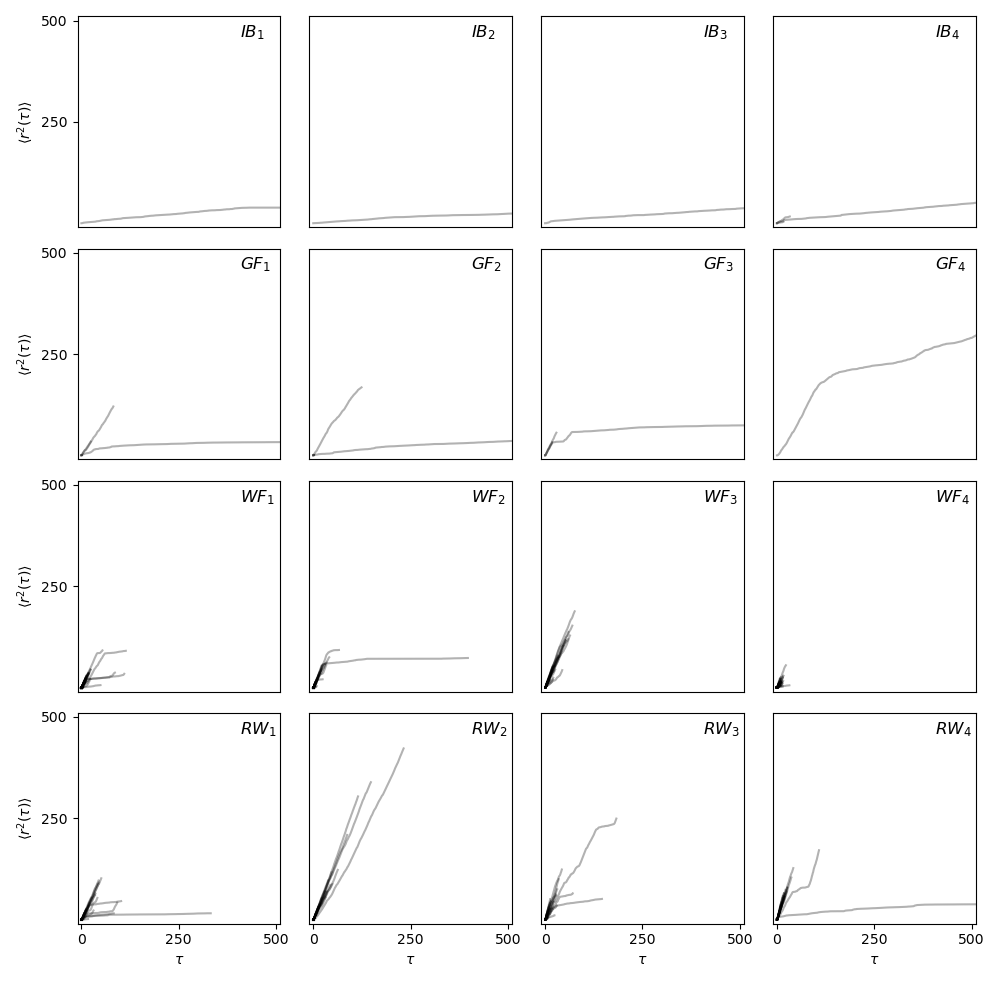
\includegraphics[width=14.7cm, height=14.7cm]{figures/MSD_branches_BW.png}}
    \caption{Depiction of the segmented $SMSD$: the resulting single branches all start at point zero, each triggered by an entry into an area that lies within a ``wall zone'', where the bees distance from the center of the arena is $r > 29$ centimeters. The opacity of each branch was reduced to 0.5 to show overlapping lines as gradations of grey. The example bees $IB_{1-4}$ show clearly and exclusively low values for the diffusion coefficient, $GF_{1-4}$ with only a few branches with a high diffusivity followed by sitting and low diffusivity. Distinction between $WF_{1-4}$ and $RW_{1-4}$ is difficult as both show numerous branches with slopes $>2$ but are showing inconsistent mixtures of high and low diffusion coefficients, where additionally big amounts of the trajectory are not taken into account.}
    \label{fig:MSD_branches_BW}
\end{figure}



\newpage
\section{Time Averaged Mean Squared Displacement $TMSD$}
\label{sec:TMSD}

Another way to look at the MSD is through a time averaged method ($TMSD$) as described in equation \ref{eq:MSD_int}.

In figure \ref{fig:MSD_lin_fit} the $TMSD$ for our 16 examples allows a first tangible analysis of the translational diffusion coefficient $D$. If we keep our initial definition of the different behaviour types, we can extract their respective values for $D$ in $n=2$ dimensions following the relation 

\begin{equation}
    \label{eq:Diff_Relation}
    TMSD \equiv \langle r^{2}(\tau) \rangle = 2nD\tau \implies m=\frac{\langle r^{2}(\tau) \rangle}{\tau}=2nD
\end{equation}

via a linear fit for $m$ and timescales $\tau$ shorter than $20$ seconds, which is the time a bee would need to traverse a distance of $60$ centimeters (i.e. the arena diameter) with a velocity of $3cm/s$. \cite{nouvian2019}

\begin{figure}%[H]
    \centering
        \frame{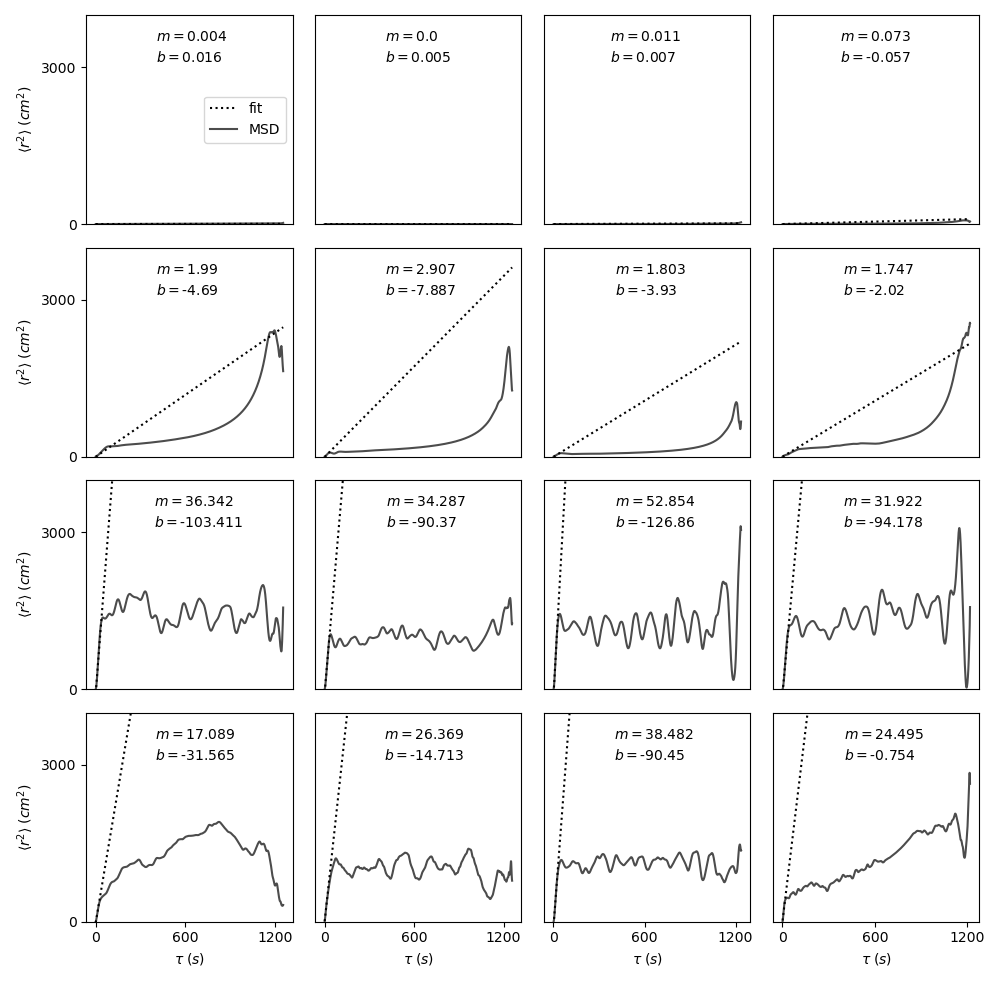
\includegraphics[width=14.7cm, height=14.7cm]{figures/lin_fit_MSD.png}}
    \caption{TSMDs of the 16 exemplary bees on a double linear scale. Only timescales $\tau < 20s$ are considered to acquire the diffusion coefficient, as this is the time a bee would theoretically need to cross the arenas diameter of $60cm$ with a velocity of $3cm/s$. The dotted line represents that linear fit for all timescales ranging in $0s<\tau<20s$. As expected the $IB_{1-4}$ show no slope at all, $GF_{1-4}$ show slopes ranging in $1.7 < m < 2.9$. $WF_{1-4}$ and $RW_{1-4}$ have slopes that are greater by a magnitude, indicating strong diffusive behaviour for short timescales at least.}
    \label{fig:MSD_lin_fit}
\end{figure}

As this diffusion coefficient flows into the noise term of equation \ref{eq:Langevin_reduce}, which affects the movement only on an infinitesimal scale $dt$, the rest ($\tau > 20s$) of the resulting MSD analysis is not of further interest in regards of the diffusion. Although noteworthy are the different slopes and forms of the MSD graphs, allowing a separation between the different types of behaviour. Immobility, represented by trajectories $IB_{1-4}$, is identified through a slope $m \approx 0.022$, and uphill movement, or trajectories $GF_{1-4}$, through a mean initial slope of $m \approx 2.112$. The distinction between $RW$ and $WF$ trajectories is again not as easily done, although $WF_{1-4}$ show oscillations in the MSD. Their slopes, although distinctly higher than with $IB_{1-4}$ or $GF_{1-4}$, have a mean value of $m \approx 38.851$ for $WF$ and $m \approx 26.609$ for $RW$ behaviour. As the slope of the $TMSD$ equals $2 n D$ with $n$ being the spatial dimensions of the tracked path, we get following values for $D$:

\begin{center}
\vspace{-2mm}
\begin{table}[H]
\caption{Translational diffusion coefficient $D$ for the different behavioural types acquired considering the slope $m$ (see figure \ref{fig:MSD_lin_fit}). The type specific diffusion coefficients only represent four bees each, the average value represents all 120 valid experiments (excluding the control sets).}
    \centering
    \begin{tabular}{p{1.2cm}|p{3.8cm}|p{4.0cm}}
         %\hline
         \textbf{Type} & \textbf{Diffusion coefficient $D$} & \textbf{Deviation $\sigma$} \\
         \hline
         \hline
         $IB_{1-4}$ & $0.006 \,cm^{2}/s$ & $\pm$ $0.030 \,cm^{2}/s$  \\
         %\hline
         $GF_{1-4}$ & $0.528 \,cm^{2}/s$ & $\pm$ $0.117 \,cm^{2}/s$  \\
         %\hline
         $WF_{1-4}$ & $9.713 \,cm^{2}/s$ & $\pm$ $2.059 \,cm^{2}/s$  \\
         %\hline
         $RW_{1-4}$ & $6.652 \,cm^{2}/s$ & $\pm$ $1.921 \,cm^{2}/s$  \\
         %\hline
         average & $2.815 \,cm^{2}/s$ & $\pm$ $3.391 \,cm^{2}/s$ \\
         %\hline
    \end{tabular}
    \label{tab:D_slope}
    \vspace{-10mm}
\end{table}
\end{center}

%\begin{center}
%    \begin{tabular}{ |p{4cm}|  }
%    \hline
%        \multicolumn{1}{|c|}{Diffusion Coefficients through slope $m$} \\
%    \hline
%        \multicolumn{1}{|c|}{$D_{IB} =0.006$} \\
%        \multicolumn{1}{|c|}{$D_{GF} = 0.528$} \\
%        \multicolumn{1}{|c|}{$D_{WF} = 9.713$} \\
%        \multicolumn{1}{|c|}{$D_{RW} = 6.652$} \\
%        \multicolumn{1}{|c|}{$D_{avg} = xx.xxx TODO$} \\
%    \hline
%    \end{tabular}
%\end{center}

\begin{figure}%[H]
    \centering
        \frame{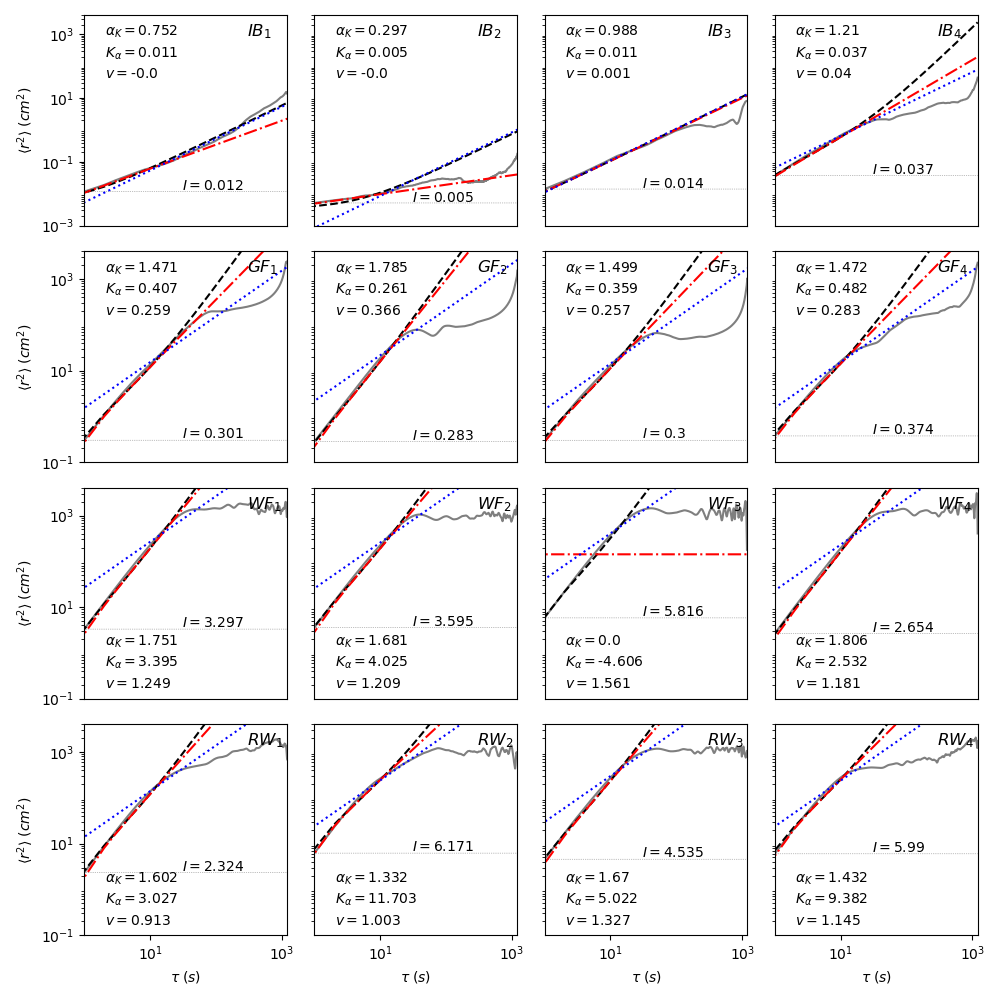
\includegraphics[width=14.7cm, height=14.7cm]{figures/2021_12_15_lin_poly_expfit_MSD_timeavg_16.png}}
    \caption{Different fits for timescales up to $20$ seconds of displacement for the 16 exemplary bees. The dotted blue line is the same linear fit that is shown in figure \ref{fig:MSD_lin_fit}. The red dash-dotted line represents a fit of a power law $\tau^{\alpha_{K}}$ to the data to show that in the logarithmic depiction a power law fits in fact better than the linear fit, showing that the diffusion taking place (if there is one at all) is a highly anomalous and super-diffusive one with $\alpha_{K}>1$ throughout all bees other than $IB_{1-4}$. The dashed black line corresponds to the quadratic term in equation \ref{eq:Diff_Relation_poly}, attempting to allow the extraction of the velocity $v$ for section \ref{sec:theta_and_velocity}. Finally, the horizontal black dotted and gently drawn line marks the intersect $I$ with the $y$-axis at $x=1$, resulting in another way to acquire the general diffusion coefficient. Additionally the values for $K_{\alpha}$ from equation \ref{eq:Diff_Relation_anomalous} are given as well.}
    \label{fig:Lin_Poly_Exp_fit}
\end{figure}

Looking at the double logarithmic plot (figure \ref{fig:Lin_Poly_Exp_fit} it is obvious that the $TMSD$ again follows a linear slope for $\tau < 10s$ and thereby implies the existence of a power law relationship up until there. This anomalous diffusive behaviour requires a different approach for the derivation of the diffusion coefficient following the relation

\begin{equation}
    \label{eq:Diff_Relation_anomalous}
    \langle r^{2}(\tau) \rangle = 2n K_{\alpha} \tau^{\alpha_{K}}
\end{equation}

where $K_{\alpha}$ is a ``generalized'' diffusion coefficient and $\alpha_{K}$ an ``anomaly parameter''. This allows for an introduction of an time dependent diffusion coefficient \cite{Metzler2000} formulated as

\begin{equation}
    \label{eq:Time_Dep_Diff_Coeff}
    D_{\alpha}(\tau) = K_{\alpha} \tau^{\alpha_{K}-1}
\end{equation}

which, put another way, introduces a ``memory'' to the system where the already elapsed trajectory has an influence on the current movement.

Although the existence of such a power law and time dependent diffusion coefficient seems to be ascertained, this approach reaches beyond the presented work and might be interesting for a separate analysis. The values for $K_{\alpha}$ are still included in figure \ref{fig:Lin_Poly_Exp_fit} and show a difference in their value, differing by an order of magnitude between $IB_{1-4}$ and $GF_{1-4}$, as well as between $GF_{1-4}$ and $WF_{1-4}$/$RW_{1-4}$. Other than that, the double logarithmic plot offers the possibility to derive the diffusion coefficient from equation \ref{eq:Diff_Relation} by locating the point of the $TMSD$ at $\tau=1$, in other words, the intersection between the $TMSD$ and the $y$-axis via the relation $I \coloneqq ln(\langle r^{2} \rangle) = ln(4D\tau)$.

%Although the existence of such a power law may be true for exemplary trajectories it must be remembered, that this can be deceiving in the end, as already small fluctuations towards the lower spectrum of the $TMSD$ can lead to a curvature of the graph, and therefore to an actually non-linear relationship. Other than that, the double logarithmic plot offers the possibility to derive the diffusion coefficient from equation \ref{eq:Diff_Relation} by locating the intersection between the $TMSD$ at $x =1$ and the $y$-axis in figure \ref{fig:Lin_Poly_Exp_fit}.

\begin{center}
\vspace{-2mm}
\begin{table}[H]
\caption{Translational diffusion coefficient $D$ for the different behavioural types acquired considering the intersect with the $y$-axis (see figure \ref{fig:Lin_Poly_Exp_fit}). The type specific diffusion coefficients represent only four bees each, the average value represents all 120 valid experiments (excluding the control sets).}
    \centering
    \begin{tabular}{p{1.2cm}|p{3.8cm}|p{4.0cm}}
         %\hline
         \textbf{Type} & \textbf{Diffusion coefficient $D$} & \textbf{Deviation $\sigma$} \\
         \hline
         \hline
         $IB_{1-4}$ & $0.017 \,cm^{2}/s$ & $\pm$ $0.012 \,cm^{2}/s$  \\
         %\hline
         $GF_{1-4}$ & $0.315 \,cm^{2}/s$ & $\pm$ $0.035 \,cm^{2}/s$  \\
         %\hline
         $WF_{1-4}$ & $3.841 \,cm^{2}/s$ & $\pm$ $1.190 \,cm^{2}/s$  \\
         %\hline
         $RW_{1-4}$ & $4.755 \,cm^{2}/s$ & $\pm$ $1.540 \,cm^{2}/s$  \\
         %\hline
         average & $1.507 \, cm^{2}/s$ & $\pm$ $1.725 \,cm^{2}/s$  \\
         %\hline
    \end{tabular}
    \label{tab:D_inter}
    \vspace{-10mm}
\end{table}
\end{center}

%\begin{center}
%    \begin{tabular}{ |p{4cm}|  }
%    \hline
%        \multicolumn{1}{|c|}{Diffusion Coefficients through intersect} \\
%    \hline
%        \multicolumn{1}{|c|}{$D_{IB} = 0.017$} \\
%        \multicolumn{1}{|c|}{$D_{GF} = 0.315$} \\
%        \multicolumn{1}{|c|}{$D_{WF} = 3.841$} \\
%        \multicolumn{1}{|c|}{$D_{RW} = 4.755$} \\
%        \multicolumn{1}{|c|}{$D_{avg} = 1.507$} \\
%    \hline
%    \end{tabular}
%\end{center}

When all the trajectories are analysed at once, the sole distribution of numerous $TMSD$ curves indicates that for short timescales $\tau < 20$ seconds the bees mostly show diffusive behaviour. The comparison of $D_{avg}$, acquired through equation \ref{eq:Diff_Relation}, and $\alpha_{K}$, which flows into equation \ref{eq:Diff_Relation_anomalous}, is illustrated in figure \ref{fig:MSD_timeavg_ALL}.

We conclude, that a diffusion coefficient $D$ which is fitted up until $\tau<20s$ is a good way to differentiate between $IB$-, $GF$- and generally random behaviour. In contrast, it is not possible to distinctly attribute a random behaviour to either the $WF$ or the $RW$ subtype.
However, bees do not move in a purely diffusive manner, even when accounting for the confinement or ballistic regime, which renders the diffusion coefficient $D$ ill defined.
A solution to that issue could be the time dependent diffusion coefficient $K_{\alpha}$ which at a first glance delivers at least the same distinction between $IB$, $GF$ and $WF/RW$. 

\begin{figure}
    \centering
    \frame{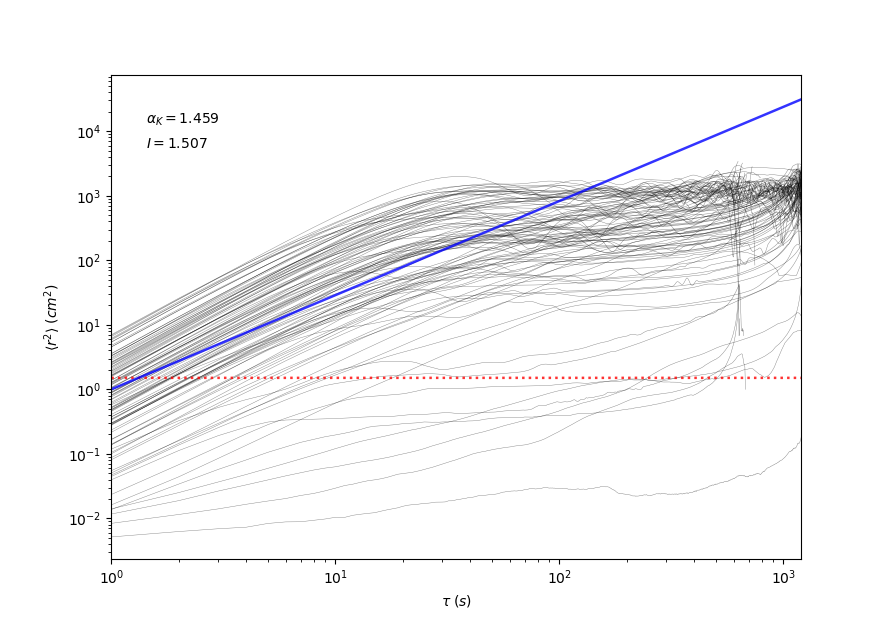
\includegraphics[width=10.7cm, height=7.66cm]{figures/2021_12_14_fit_MSD_timeavg_ALL.png}}
    \caption{Layered $TSMDs$ of all experiments with a reduced opacity in a double logarithmic plot. $\alpha_{K}$ is hereby the averaged exponent of a power law $\tau^{\alpha_{K}}$ (blue solid) and $I$ (red dotted) the average intersection with the $y$-axis at $x=0$.} 
    \label{fig:MSD_timeavg_ALL}
\end{figure}

\newpage


\section{Analysis of Angle $\theta$ and Velocity $v$}
\label{sec:theta_and_velocity}
\subsubsection{Velocities}

Revisiting equation \ref{eq:Diff_Relation} and expanding it by a quadratic term $(v \tau)^{2}$, results in a polynomial 

\begin{equation}
    \label{eq:Diff_Relation_poly}
    \langle r^{2}(\tau) \rangle = (v \tau)^2 + 2nD\tau
\end{equation}

from which we can generally derive the velocity as well (see figure \ref{fig:Lin_Poly_Exp_fit}) \cite{Tseng2002} \cite{Cherstvy2021}. Fitting the polynomial to $\tau>20s$ is hereby not resulting in any proper information, which is the reason that again only timescales of $0<\tau<20$ seconds were analysed. Hereby the initial velocities for the immobile bees $IB_{1-4}$ lie at zero centimeters per second as expected, for $GF_{1-4}$ at around $0.3cm/s$ and for $WF_{1-4}$ and $RW_{1-4}$ in a comparably wider span, ranging from $1cm/s$ to $1.5cm/s$.

\begin{center}
\vspace{-2mm}
\begin{table}[H]
\caption{Mean walking velocity for the different behavioural types acquired through the fit of the polynomial (see figure \ref{fig:Lin_Poly_Exp_fit}). The mean velocities represent four bees each.}
    \centering
    \begin{tabular}{p{1.2cm}|p{3.0cm}|p{4.0cm}}
         %\hline
         \textbf{Type} & \textbf{Mean velocity $v_{bee}$} & \textbf{Deviation $\sigma$} \\
         \hline
         \hline
         $IB_{1-4}$ & $0.010 \,cm/s$ & $\pm$ $0.017 \,cm/s$  \\
         %\hline
         $GF_{1-4}$ & $0.291 \,cm/s$ & $\pm$ $0.044 \,cm/s$  \\
         %\hline
         $WF_{1-4}$ & $1.300 \,cm/s$ & $\pm$ $0.153 \,cm/s$  \\
         %\hline
         $RW_{1-4}$ & $1.097 \,cm/s$ & $\pm$ $0.156 \,cm/s$  \\
         %\hline
    \end{tabular}
    \label{tab:vel_poly}
    \vspace{-10mm}
\end{table}
\end{center}

%\begin{center}
%    \begin{tabular}{ |p{4cm}|  }
%    \hline
%        \multicolumn{1}{|c|}{Velocities through polynomial} \\
%    \hline
%        \multicolumn{1}{|c|}{$v_{IB} = 0.010 \,cm/s$} \\
%        \multicolumn{1}{|c|}{$v_{GF} = 0.291 \,cm/s$} \\
%        \multicolumn{1}{|c|}{$v_{WF} = 1.300 \,cm/s$} \\
%        \multicolumn{1}{|c|}{$v_{RW} = 1.097 \,cm/s$} \\
%        \multicolumn{1}{|c|}{$v_{avg} = \,cm/s TODO$} \\
%    \hline
%    \end{tabular}
%\end{center}


\\
Another not quite as elegant but nevertheless better approach is to look at the histogram and thereby the distribution of the velocities of the whole run (see figure \ref{fig:Hist_velocity}) which will be needed in a following section for the analysis of the RTS as well. Compared with the results from before, this indicates some discrepancy at first sight, : the $IB_{1-4}$ have an even if small still nonzero velocity, for $GF_{1-4}$ it lies at $v \approx 1.5cm/s$, and for $WF_{1-4}$ and $RW_{1-4}$ it is well beyond $1.5 cm/s$. This can be attributed solely to the fact, that indeed the whole trajectory is considered. For $IB_{1-4}$ it suggests that this representation is more susceptible for the noise that is acting on the system, and that the bees do actually move at some point. 
%The histograms are additionally treated as two separate distributions, each normalized to $1$. The $GF_{1-4}$ behaviour indicates with its higher mean velocity, that it accelerates at some point after the initial $20$ seconds. Same holds true for $WF_{1-4}$ and $RW_{1-4}$, although their velocities at start were already high.
\\
Ignoring the velocities dependence on the temperature for now, and simply looking at the histograms, it is apparent that there indeed seems to be a switching between two (discrete) Poisson-distributed processes which can be continuously formulated as a exponential distribution

\begin{equation}
    f(x, \lambda) = \lambda e^{-\lambda x}
    \label{eq:Exponential_PDF} 
\end{equation}

for the velocities $v<0.5cm/s$ and as a Normal distribution 

\begin{equation}
\label{eq:Normal}
     f(x,\mu,\sigma) = \frac{1}{\sigma \sqrt{2\pi}} e^{-\frac {1}{2}\left(\frac {x-\mu }{\sigma }\right)^{2}}
\end{equation}

for velocities $v$ that are greater than $0.5cm/s$.
\\
The two distributions have each been separately normalized to 1 as only one of them acts on the bees velocity at a time.

\begin{figure}%[H]
    \centering
        \frame{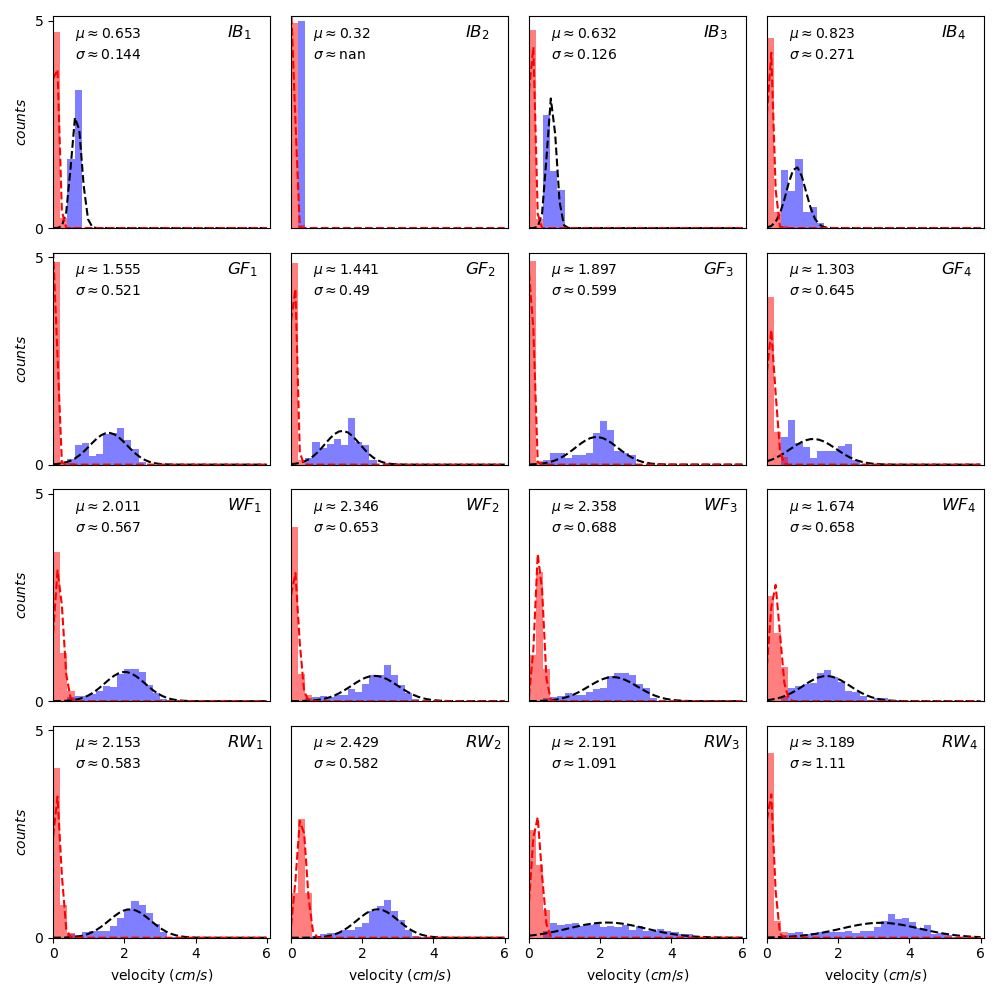
\includegraphics[width=14.7cm, height=14.7cm]{figures/Hist_velocity.png}}
    \caption{Histograms of all velocities of the 16 exemplary bees. The red bars mark all velocities $v_{bee}$ below $0.5cm/s$ for when the bee is barely moving, the blue bars depict the base velocity $v_{bee}$ greater than $0.5cm/s$, onto which a Normal distribution was fitted. The values for the mean $\mu$ and the standard deviation $\sigma$ are given for each individual run. A visible difference in velocities between the different types again allows to separate them in low ($<1cm/s$), medium ($\approx 1.5cm/s$) and high ($>2cm/s$) values.}
    \label{fig:Hist_velocity}
\end{figure}

\begin{center}
\vspace{-2mm}
\begin{table}[H]
\caption{Mean walking velocity for the different behavioural types acquired through the Gaussian fit (see figure \ref{fig:Hist_velocity}). The type specific mean velocities represent four bees each, the average value represents all 120 valid experiments (excluding the control sets).}
    \centering
    \begin{tabular}{p{1.2cm}|p{3.0cm}|p{4.0cm}}
         %\hline
         \textbf{Type} & \textbf{Mean velocity $v_{bee}$} & \textbf{Deviation $\sigma$} \\
         \hline
         \hline
         $IB_{1-4}$ & $0.607 \,cm/s$ & $\pm$ $0.018 \,cm/s$  \\
         %\hline
         $GF_{1-4}$ & $1.475 \,cm/s$ & $\pm$ $0.220 \,cm/s$  \\
         %\hline
         $WF_{1-4}$ & $2.097 \,cm/s$ & $\pm$ $0.281 \,cm/s$  \\
         %\hline
         $RW_{1-4}$ & $2.491 \,cm/s$ & $\pm$ $0.417 \,cm/s$  \\
         %\hline
         average & $1.704 \,cm/s$ & $\pm$ $0.573 \,cm/s$  \\
         %\hline
    \end{tabular}
    \label{tab:vel_gauss}
    \vspace{-10mm}
\end{table}
\end{center}

%\begin{center}
%    \begin{tabular}{ |p{4cm}|  }
%    \hline
%        \multicolumn{1}{|c|}{Velocities through normal distribution} \\
%    \hline
%        \multicolumn{1}{|c|}{$v_{IB} = 0.607 \,cm/s$} \\
%        \multicolumn{1}{|c|}{$v_{GF} = 1.475 \,cm/s$} \\
%        \multicolumn{1}{|c|}{$v_{WF} = 2.097 \,cm/s$} \\
%        \multicolumn{1}{|c|}{$v_{RW} = 2.491 \,cm/s$} \\
%        \multicolumn{1}{|c|}{$v_{avg} = TODO \,cm/s$} \\
%    \hline
%    \end{tabular}
%\end{center}

The behaviour of the velocities in presence of a gradient can as well be investigated by looking at its power spectral density $S_{v}$ over frequency domain $\omega$ (see equation \ref{eq:PSD_velocity} and figure \ref{fig:PSD_velocity}). As a flattening of the PSD and $a_{\theta} > 0$ is only recognisable in $GF_{1-4}$, this indicates that their velocities are most effectively governed by the temperature. The decrease over $1/\omega^{\alpha_{pow}}$ is present in all of them, and ranges for exponents $0<\alpha_{pow}<3$, which reveals Gaussian white noise at $\alpha_{pow}=0$ and Brownian motion at $\alpha_{pow}=2$ at high frequencies. Finally, due to the fact that most of the PSD show a decrease looking more like $1/\omega$, for which there are many explanations with the random telegraph or ``flicker'' noise from section \ref{sec:RTS} being one of them, a general dependence on the temperature can be attributed to all of the exemplary bees, excluding the immobile ones.

In conclusion it can be stated that equation \ref{eq:PSD_velocity} is a poor fit for the power spectral density $S_{v}$, meaning that $v_{0}(t)$ is not governed by noise around a characteristic mean velocity $v_{bee}$, but rather switches between velocities $v=0$ and $v_{bee}>0$.

\begin{figure}%[H]
    \centering
        \frame{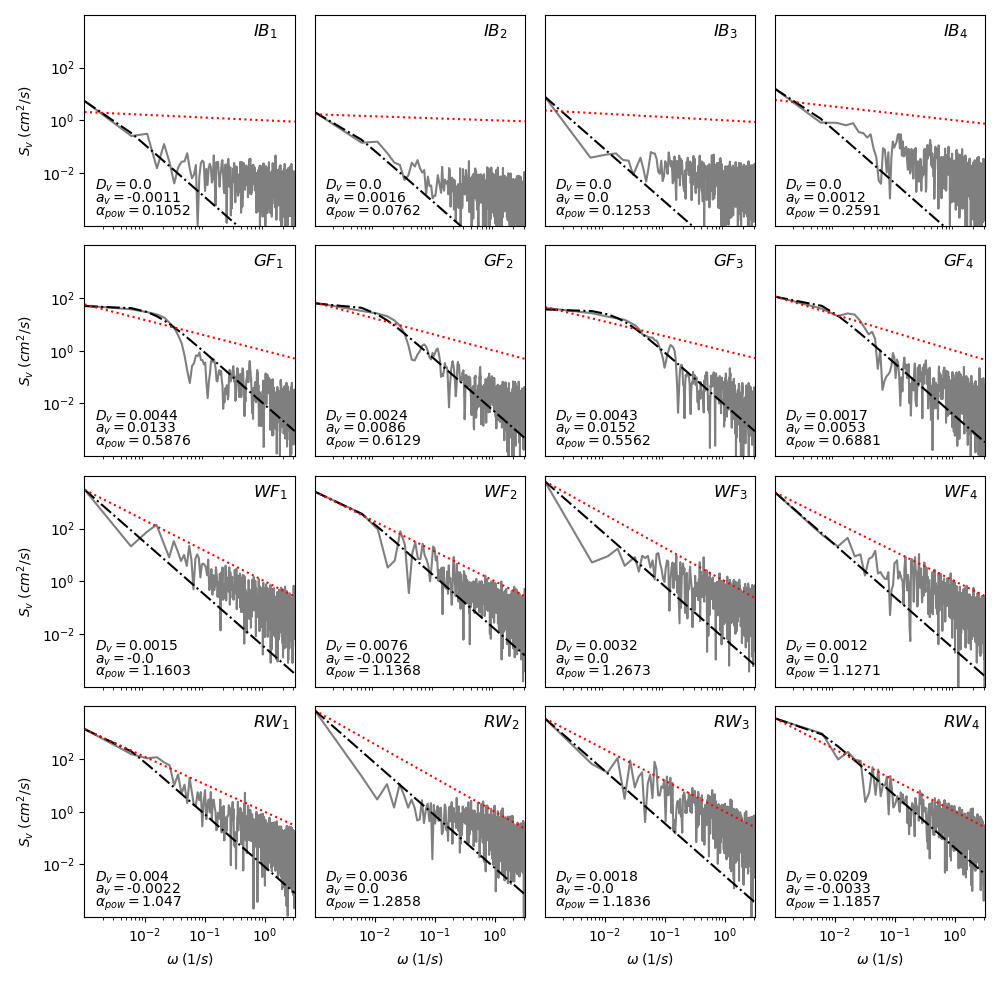
\includegraphics[width=14.7cm, height=14.7cm]{figures/PSD_velocity.png}}
    \caption{PSD of the velocity for the 16 exemplary bees, acquired through equation \ref{eq:PSD_velocity} for the dash-dotted line, representing the analytical fit for $D_{v}$ and $a_{v}$. The solid grey line depicts the PSD of the experimental data acquired through its Fourier-transformed signal. For low frequencies $\omega$ we generally see a decrease following $1/\omega^{2}$ that then switches to something more resembling a decrease proportional to $1/\omega$, meaning that first there is no influence of the temperature on the velocities followed by $\omega$ where a dependence seems possible, which may be induced by a stopping and walking behaviour. Regarding the velocities of $GF_{1-4}$ it is apparent that there is a cutoff frequency, suggesting a considerably high dependency on temperature for low $\omega$. This cutoff, even if less pronounced, is present in $WF_2$ or $RW_4$ as well, which makes sense as those particular two bees did spend a lot of time with $v=0cm/s$ in the optimum, confirming this approach in general but failing to deliver useful information for the rest of the $RW$ and $WF$ bees. What it does deliver though, is the fact that a distinction between less and more active behaviour is possible by looking at the intersect with the $y$-axis.}
    \label{fig:PSD_velocity}
\end{figure}

In the context of velocity, its general dependency on the local temperature needs to be investigated as well (see figure \ref{fig:vel_vs_dT}), as this relation is required for the drift term in equation \ref{eq:Langevin_reduce}. It is evident that the dependency is an approximately linear one, with on average higher velocities for lower temperatures and vice versa ($2.5cm/s$ at $28^{\circ}C$ and $1.0cm/s$ at $36^{\circ}C$).

\begin{figure}%[H]
    \centering
        \frame{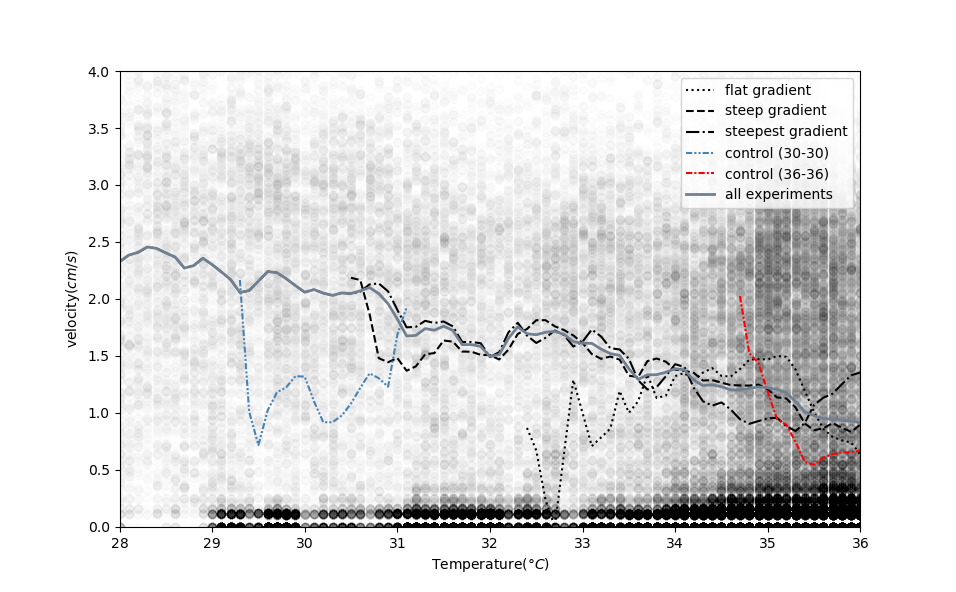
\includegraphics[width=14.7cm, height=8.7cm]{figures/2022_01_11_mean_bin_vel_vs_dT_split_grad.png}}
    \caption{Temperature dependent velocity. The background shows all velocities in all points in time of all bees. The dotted line considers only experiments with a flat gradient of around $2^{\circ}C$, the dashed line only experiments with a steeper gradient of around $4^{\circ}C$ and the dash-dotted line the steepest gradients. The solid grey line (and foundation for the linear fit) represents the mean of all experiments at all temperatures with a resolution of $0.1^{\circ}C$. The blue dash-dotted line are the control experiments, where both, optimum and sub-optimum were set to $30^{\circ}C$, similarly the red dash-dotted line consists of the corresponding control experiments at $36^{\circ}C$. The slope $b$ of the linear fit to the mean curve equals to $b=3/16$.}
    \label{fig:vel_vs_dT}
\end{figure}

\subsubsection{Turning Angle $\theta$}

To determine the values for $a_{\theta}$ and $D_{\theta}$ from equation \ref{eq:PSD_theta}, the respective PSD was modeled and fitted to the experimental data (see \ref{fig:PSD_angle}).
The fit shows a drop that is proportional $1/\omega^{2}$ for high $\omega$ in all of them, which was expected. The fact that their cutoff frequencies are randomly distributed however supports the surprising interpretation that the bees are not that thoroughly turning into the direction of highest gradient ascent. In other words, bees behave less based on the concept of ``colder'' or ``warmer than before'', but rather on ``warm enough''. %(which, as we will see, then can trigger a stopping event).

\begin{figure}%[H]
    \centering
        \frame{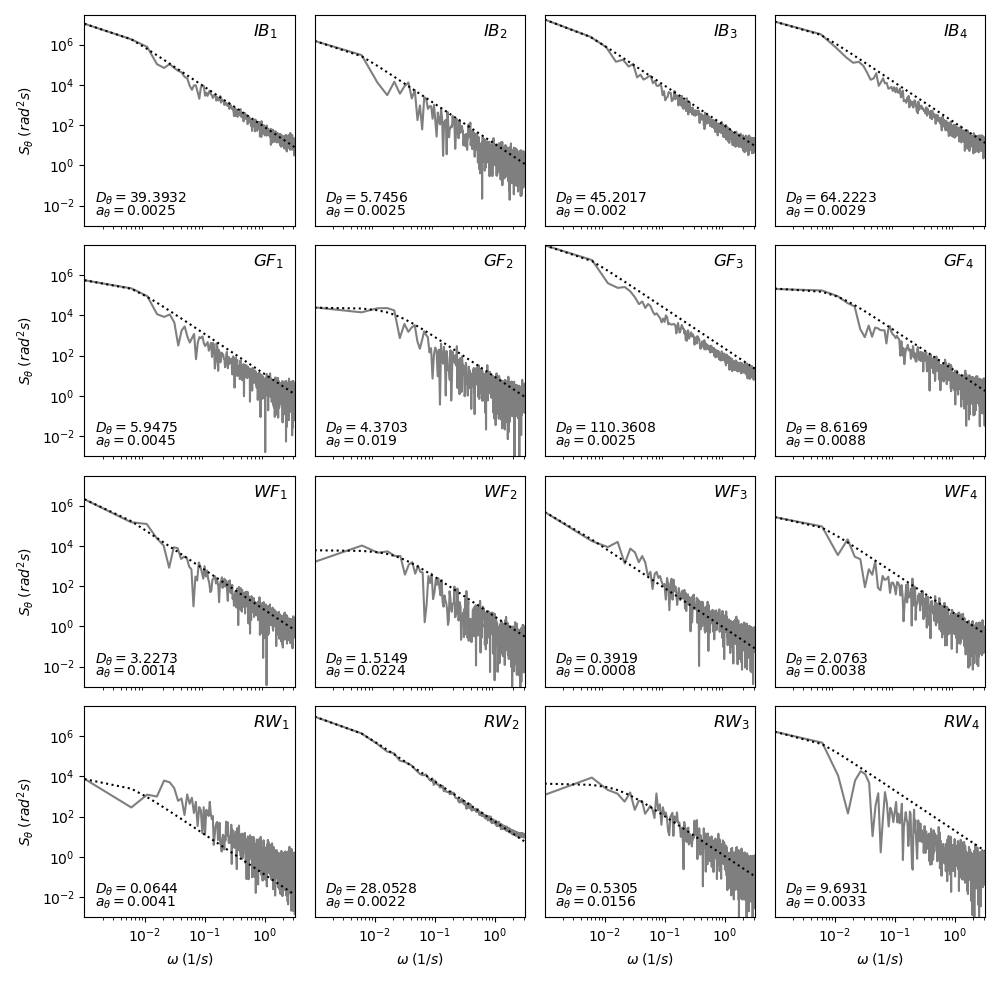
\includegraphics[width=14.7cm, height=14.7cm]{figures/2021_12_07_PSD_angle_16.png}}
    \caption{The PSDs of the angle $\theta$ for the 16 exemplary bees show interesting properties: firstly, the Lorentzian shape is practically present in every spectrum,  secondly, their cutoff frequencies are not very distinct, especially when comparing $GF_{1-4}$ with $RW_{1-4}$. In general the bees reaction to the gradient is less prevalent than expected. The different noise intensities, which can be explained by different amounts of randomness acting on the angles amplitude, are not special to any of the different behaviours. Additionally observable is, that they uniformly show a $1/\omega^{2}$ dependence.}
    \label{fig:PSD_angle}
\end{figure}

%Again looking at all the experiments at once in regarding the $D_{\theta}$ and $a_{\theta}$ pairs, we see a linear dependence between them, which seems sensible at a first glance as a bee that moves/turns a lot is more likely to find the goal (see figure \ref{fig:D_vs_a_theta}).

\begin{figure}%[H]
    \centering
        \frame{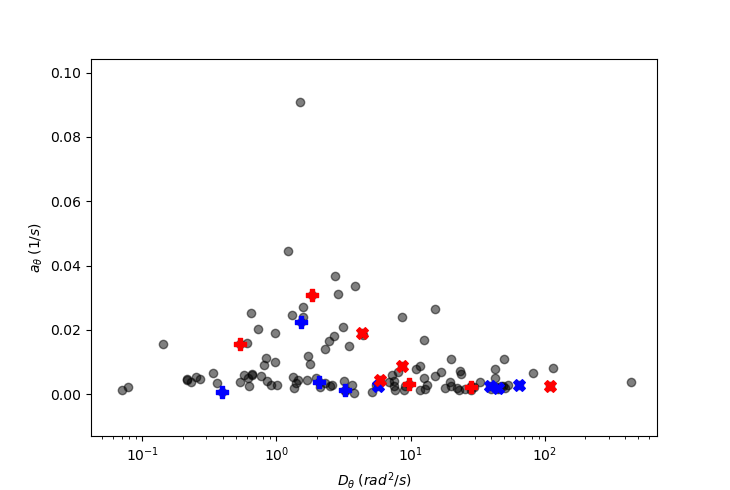
\includegraphics[width=11.5cm, height=7.5cm]{figures/2021_12_08_scatter_D_vs_a.png}}
    \caption{Values of $D_{\theta}$ plotted over $a_{\theta}$ for all bees. The red ``X'' markers stand for $IB_{1-4}$, the red ``+'' for $GF_{1-4}$, the blue ``X'' mark $WF_{1-4}$ and the blue ``+'' mark $RW_{1-4}$. The two values seem to be uncorrelated, however When looking at the plot in single logarithmic depiction ($log($x$)$), the aggregated $D_{\theta}$ over $a_{\theta}$ resemble a Log-normal distribution.}
    \label{fig:D_vs_a_theta}
\end{figure}

\newpage

\section{Analysis of the RTS}

%It was already shown, that there is an apparent switching between some type specific mean walking speed $v_{bee}$ and a velocity $v \approx 0$ (see figure \ref{fig:Hist_velocity}).

To see whether our assumptions regarding the switching behaviour between walking and stopping again follows a $1/\omega^{\alpha_{RTS}}$ decrease, and if $\alpha_{RTS}$ differs between the types, we will continue by analysing the power spectrum of the random telegraph signal as described in equation \ref{eq:PSD_RTS}.

%For that we will first try to find the average times $t_{s}$ and $t_{w}$ and their possible dependence on the temperature $T$.

For our 16 exemplary behaviour types we have already seen in figure \ref{fig:Hist_velocity} that there is a clear dominance of two uncorrelated Poisson-distributed and type specific velocities $v = v_{bee}$ and $v = 0$. To determine the mean velocity $v_{bee}$ it is sufficient to fit a continuous Gaussian distribution to the histograms velocities above $0.5 cm/s$, for as the Poisson distribution is only given for discrete values. All velocities below $0.5 \,cm/s$ are considered to be sitting as they lie just below the mean velocity for the bees that show immobile behaviour (see table \ref{tab:vel_gauss}).

%To see whether a random walking bee actually exhibits a change in velocity that can be compared to a random telegraph signal, a vivid example is given by bee $RW_3$ in figure \ref{fig:RTS_RW3}. It is evident that there is such a switching present in this particular experimental run, that actually has been chosen as an example for precisely this behaviour. 

To see whether the bees actually exhibit a change in velocity comparable to a RTS
When the definition of those two states is being plotted over the experimental run time, it indeed is observable that the resulting signal jumps randomly between ``0'' and ``1'', for $RW_{1-4}$ and $WF_{1-4}$ (see figure \ref{fig:RTS_second}) more so than for $IB_{1-4}$ and $GF_{1-4}$ (see figure \ref{fig:RTS_first}).

\begin{figure}%[H]
    \centering
        \frame{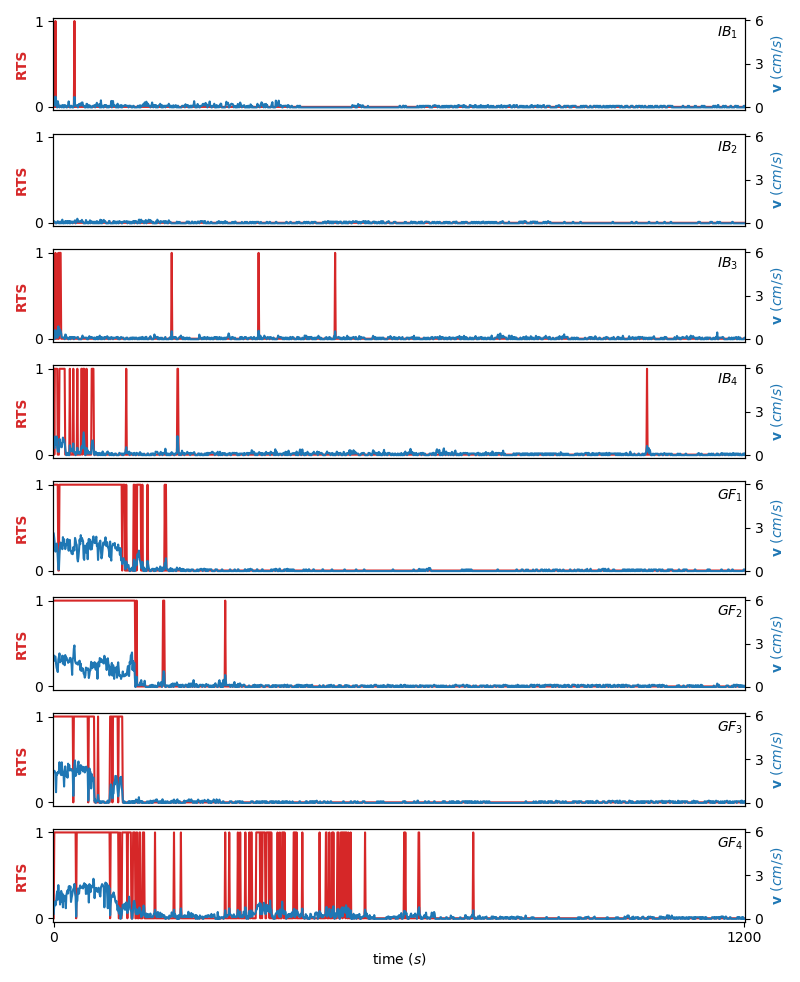
\includegraphics[width=14cm, height=18cm]{figures/2022_01_18_is_it_really_RTS_first_8.png}}
    \caption{Velocities of $IB_{1-4}$ and $GF_{1-4}$ in blue and their associated random telegraph signal in red.}
    \label{fig:RTS_first}
    \vspace{-15mm}
\end{figure}

\begin{figure}%[H]
    \centering
        \frame{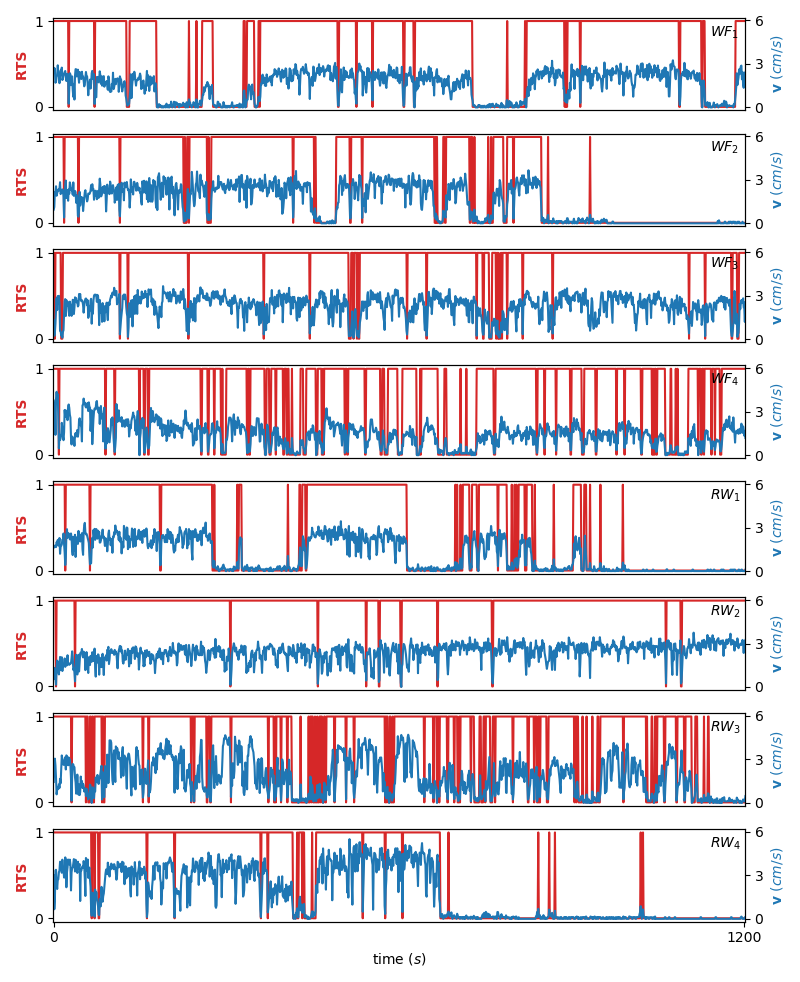
\includegraphics[width=14cm, height=18cm]{figures/2022_01_18_is_it_really_RTS_second_8.png}}
    \caption{Velocities of $WF_{1-4}$ and $RW_{1-4}$ in blue and their associated random telegraph signal in red.}
    \label{fig:RTS_second}
    \vspace{-15mm}
\end{figure}

Furthermore considering the second assumption that the duration a bee is sitting still $t_{s}$ is dependent on temperature, and the duration it walks $t_{w}$ is not, can be evaluated by looking at the correlation of $t_{s}$, $t_{w}$ and $\Delta T$ (see figure \ref{fig:ALL_stop_walk}).
$\Delta T$ is hereby the absolute difference of the local temperature $T$ at times $t_{s}$ and $t_{w}$ and the temperature at the optimum $T_{opt}$. In both cases the local temperature was defined as the mean temperature over the span of $t_{s}$ and $t_{w}$ respectively. 
Here again the recognisably different distributions indicate that the assumption holds true, the linear fit to a function $t = m \Delta T + b$ for $t_{s}$ shows a slope of $\approx -25$ whereas it is $\approx 2$ for $t_{w}$. It seems that for $t_{s}$ another function would better describe the behaviour, namely an exponential function (maybe even a power law of some sorts) and an example is given in figure \ref{fig:ALL_stop_walk} by comparing the linear fit to the fairly strong function $t = \tau \cdot e^{-\beta \Delta T}$. 

\begin{figure}%[H]
    \centering
        \frame{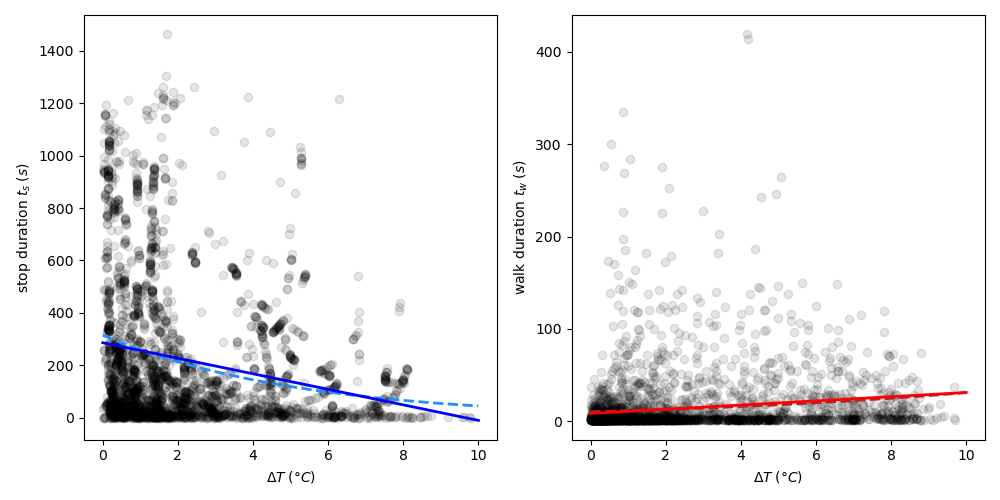
\includegraphics[width=14cm, height=6.5cm]{figures/2022_01_12_ALL_t0_t1_of_dT_scatter_nonlin_fit.png}}
    \caption{Scatter plots of the experimental stopping and walking durations $t_{s}$ (left) and $t_{w}$ (right) in dependence of the temperature $\Delta T = |T - T_{opt}|$. The blue solid line represents the linear fit, the dashed line (light blue) is a curve fit to a function $\tau \cdot e^{-\beta \Delta T}$. For higher $\Delta T$ the linear fit remains to be the better one and there seems not to be any significant improvement for lower $\Delta T$ through the exponential function. However all fits confirm what was expected: $t_{s}$ is highly temperature dependent, and $t_{w}$ is not, which is sensible, considering the fact that the $\Delta T$ for each walking duration is computed by averaging it over the span of $t_{w}$.}
    \label{fig:ALL_stop_walk}
\end{figure}

Looking at the fits of $t_{s}(\Delta T)$ for the 16 exemplary bees we see that a linear relationship would not be sufficient anymore to represent what is going on, and in this individual depiction aforementioned fit to $t = \tau \cdot e^{-\beta \Delta T}$ delivered better results (see figure \ref{fig:t_stopping_nonlin_16}) % and \ref{fig:t_stopping_nonlin_group4}).

\begin{figure}%[H]
    \centering
        \frame{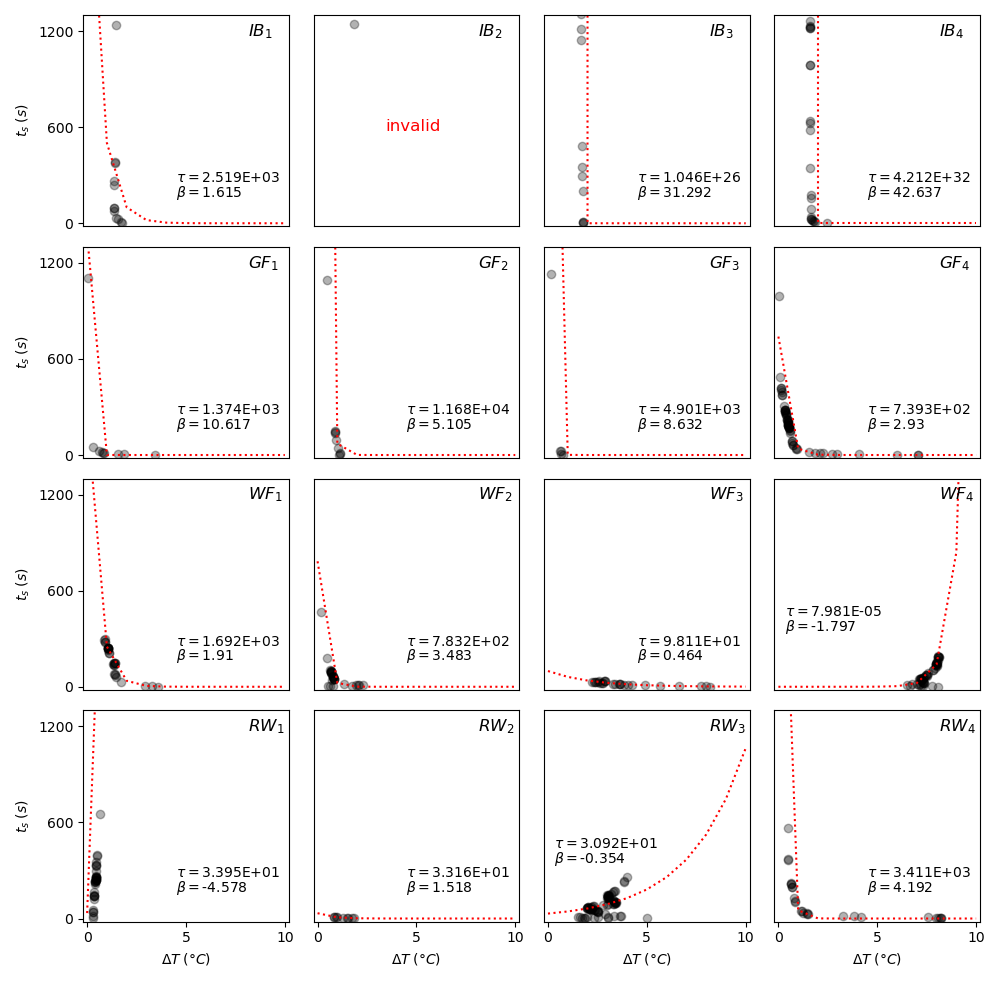
\includegraphics[width=14.7cm, height=14.7cm]{figures/2022_01_13_RTS_PSD_16_nonlin_fit.png}}
    \caption{Individual fittings for $t_{s}$ for the 16 exemplary bees. $IB_{2}$ has only a single point of data, a curve fit leads to undefined values. Note that $IB_{1-4}$ were experiments with a flat gradient of $\Delta T_{max} \approx 2^{\circ} C$, the bees have practically an infinitely high $t_{s}$ at the $\Delta T$ they have been released into the arena. $GF_{1-4}$ show low $t_{s}$ at any $\Delta T$ that is not near the optimum. $WF_{1-4}$ and $RW_{1-4}$ again are fairly random whereas there still exists a tendency towards longer stopping durations at temperatures nearer to the optimum. The red dotted line depicts the fit responding to the curve $t = \tau \cdot e^{-\beta \Delta T}$ with their individual parameters $\tau$ and $\beta$.} 
    \label{fig:t_stopping_nonlin_16}
\end{figure}

%\begin{figure}%[H]
%    \centering
%        \frame{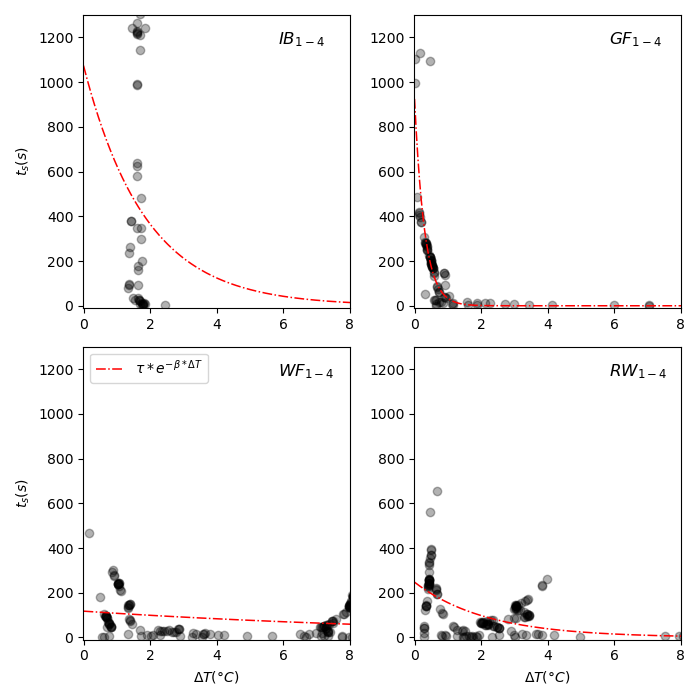
\includegraphics[width=10.7cm, height=10.7cm]{figures/2022_01_14_RTS_PSD_nonlin_fit_of_t0_group_4_V2.png}}
%    \caption{To see whether a bigger set of points leads to a clearer picture, the four individual trajectories for each type of behaviour have been grouped and $t_{s}$ is shown for each of the four types of behaviour. The red dash-dotted line depicts the fit responding to the curve $t = \tau \cdot e^{-\beta \Delta T}$ with their individual parameters $\tau$ and $\beta$. Unfortunately such a grouping is not useful in this particular case with the chosen experiments. One reason surely lies in the different gradients - the examples were initially chosen solely based on the appearance of their trajectory without other information, another one in the low number of representing experiments used. Nevertheless, the dependence is again visible and strongest in $GF_{1-4}$.} 
%    \label{fig:t_walking_nonlin_group4}
%\end{figure}

Finally, after acquiring $t_{s}$ and $t_{w}$ we can now look at the power spectra of the telegraph signals (see figure \ref{fig:RTS_PSD_16}). It is noticeable that the experimental power spectrum is only partially comparable to the analytically derived function (equation \ref{eq:PSD_vivj}). Looking at its slopes for higher $\omega$ we see that it fits best for individuals that actually experience a pronounced random telegraph signal ($WF_1$, $WF_4$, $RW_3$). In general it fits well enough for most of them, it is however partially too steep and therefore misleading: looking at $RW_2$, the fit of equation \ref{eq:PSD_vivj} suggests that there is a fairly strong switching happening, when it is known that this bee rarely sits, hence delivering not enough data points to be expressed like that. This gives rise to the questions firstly, whether there is another way of representing the switching behaviour needed, and secondly whether the data would require additional filtering.

\begin{figure}%[H]
    \centering
        \frame{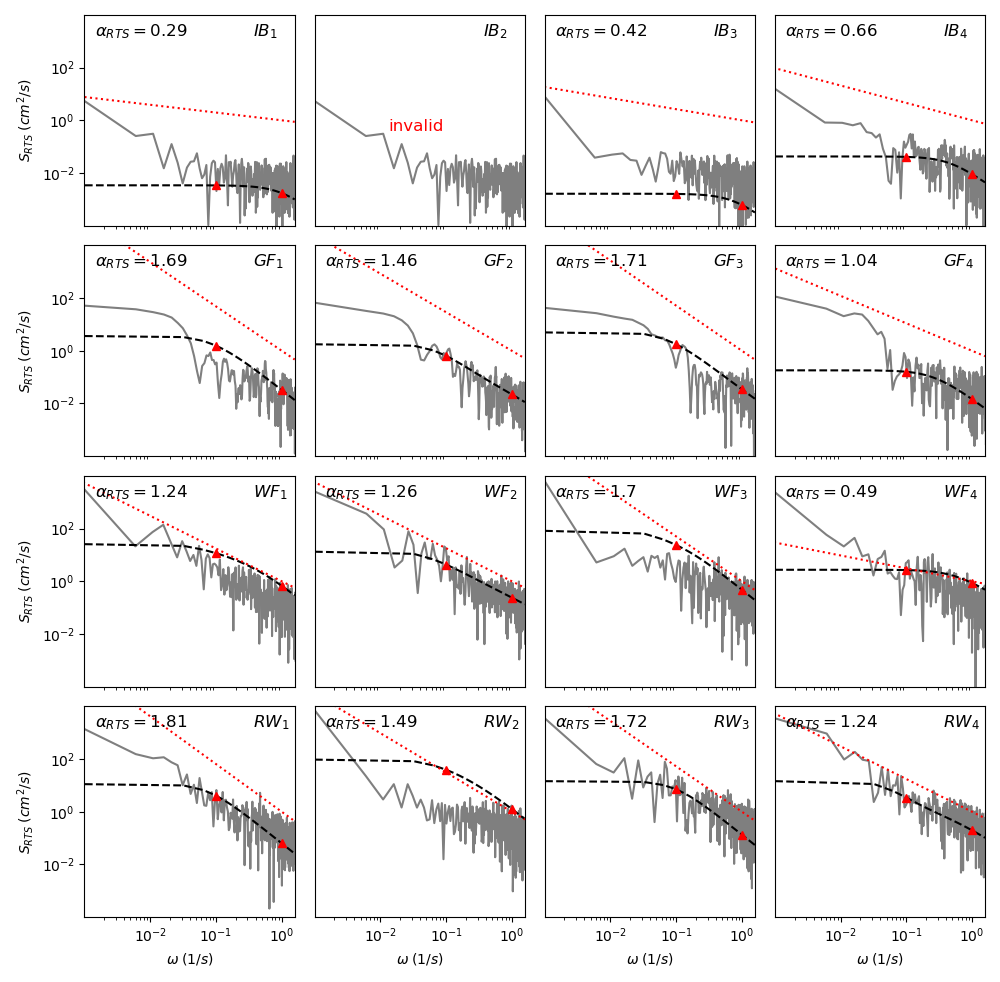
\includegraphics[width=14.7cm, height=14.7cm]{figures/2022_01_16_RTS_PSD_16.png}}
    \caption{Experimental power spectrum of the velocity (grey solid) and the analytical description of the RTSs spectrum (black dashed). The space in between the red triangles mark one order of magnitude from $10^{-1}$ to $10^0$. The red dotted line stands for a $1/\omega^{\alpha}$ relation where $\alpha_{RTS}$ is the decrease of $S_{RTS}$ over aforementioned span, given in orders of magnitude.}  
    \label{fig:RTS_PSD_16}
\end{figure}

To be able to look at all bees and all fitted values at once and see if there are similarities or patterns that let us compare them again with the subjectively and manually assigned types, everything is collectively presented in table \ref{tab:AllData}.

\begin{table}
\caption{
\textbf{ID}: experiment identification $\: |$
$\mathbf{\nabla V}$: type of gradient (1:flat, 2:steep, 3:steepest) $\: |$
\textbf{type}: manual classification $\: |$
$\mathbf{D_{TMSD}}$: see section \ref{sec:TMSD} $\: |$
$\mathbf{v_{TMSD}}$: see equation \ref{eq:Diff_Relation_poly} $\: |$
$\mathbf{K}_{\boldsymbol{\alpha}}$: time dependent diffusion coefficient $\: |$
$\boldsymbol{\alpha}_\mathbf{{K}}$: exponent corresponding to $K_{\alpha}$ $\: |$ 
$\mathbf{v_{bee}}$: mean walking velocity, see equation \ref{eq:Normal} $\: |$
$\mathbf{D_{v}}$: see equation \ref{eq:PSD_velocity} $\: |$
$\mathbf{a_{v}}$: see equation \ref{eq:PSD_velocity} $\: |$
$\boldsymbol{\alpha_{pow}}$: exponent corresponding to power law $1/\omega^{\alpha}$
$\mathbf{D}_{\boldsymbol{\theta}}$: see equation \ref{eq:PSD_theta} $\: |$
$\mathbf{a}_{\boldsymbol{\theta}}$: see equation \ref{eq:PSD_theta} $\: |$
$\boldsymbol{\tau}$ and $\boldsymbol{\beta}$: corresponding to the fitting function $\tau \cdot e^{-\beta \Delta T}$ $\: |$
$\boldsymbol{\alpha_{RTS}}$: exponent corresponding to method used in figure \ref{fig:RTS_PSD_16} $\: |$

}
\label{tab:AllData}
\resizebox{\textwidth}{!}{%
%\begin{adjustbox}{angle=90}
\begin{tabular}{l|c|l|l|l|l|l|l|l|l|l|l|l|l|l|l}%
    \bfseries ID & $\nabla V$ & type & $D_{TMSD}$ & $v_{TMSD}$ & $K_{\alpha}$ & $\alpha_{K}$ & $v_{bee}$ & $D_{v}$ & $a_{v}$ & $\alpha_{pow}$ & $D_{\theta}$ & $a_{\theta}$ & $\tau$ & $\beta$ & $\alpha_{RTS}$\\
    \hline
    \hline
    \bfseries BT01A-1 & 1 & IB & 0.3075 & 0.22 & 0.22 & 1.54 & 1.02 & 0.0008 & 0.0053 & 0.578 & 25.5556 & 0.0016 & 2.13e+30 & 79.22 & 0.64 \\
    \bfseries BT01A-2 & 1 & IB & 1.4125 & 0.5 & 0.4 & 1.84 & 1.16 & 0.0014 & 0.0034 & 0.778 & 12.7249 & 0.0016 & 0.0 & -10.51 & 1.44 \\
    \bfseries BT01A-3 & 1 & GF & 0.145 & 0.16 & 0.08 & 1.63 & 0.94 & 0.0004 & 0.0067 & 0.35 & 1.3219 & 0.0053 & 5.45e+03 & 5.09 & 0.85 \\
    \bfseries BT01A-4 & 1 & RW & 3.3275 & 0.78 & 1.13 & 1.8 & 1.21 & 0.0006 & 0.0005 & 1.005 & 1.7855 & 0.0095 & 140.46 & 0.56 & 1.79 \\
    \hline
    \bfseries BT01C-1 & 1 & RW & 3.3975 & 0.83 & 3.16 & 1.54 & 2.49 & 0.0136 & 0.0053 & 0.993 & 0.9691 & 0.0101 & 1.02e+03 & 7.81 & 1.3 \\
    \bfseries BT01C-2 & 1 & RW & 2.975 & 0.76 & 1.93 & 1.63 & 2.36 & 0.0077 & 0.0052 & 0.919 & 1.7049 & 0.012 & 0.0 & -36.93 & 1.34 \\
    \bfseries BT01C-3 & 1 & GF & 1.42 & 0.53 & 1.0 & 1.61 & 2.52 & 0.0139 & 0.0152 & 0.729 & 0.0778 & 0.0023 & 7.10e+03 & 7.46 & 1.35 \\
    \bfseries BT01C-4 & 1 & GF & 0.5175 & 0.3 & 0.77 & 1.4 & 1.87 & 0.0078 & 0.0158 & 0.639 & 0.8132 & 0.0092 & 3.13e+07 & 32.06 & 1.06 \\
    \hline
    \bfseries BT02A-1 & 1 & IB & 0.3225 & 0.17 & 0.66 & 1.22 & 1.68 & 0.0041 & 0.0117 & 0.608 & 1.2131 & 0.0445 & 0.0 & -97.95 & 1.42 \\
    \bfseries BT02A-2 & 1 & WF & 5.5225 & 1.03 & 2.76 & 1.7 & 2.52 & 0.0179 & 0.0057 & 1.016 & 22.0984 & 0.0018 & 5.46e+08 & 90.5 & 1.43 \\
    \bfseries BT02A-3 & 1 & IB & 1.355 & 0.51 & 0.48 & 1.8 & 2.08 & 0.0065 & 0.0131 & 0.655 & 441.9584 & 0.004 & 2.79e+04 & 4.01 & 1.78 \\
    \bfseries BT02A-4 & 1 & GF & 1.6875 & 0.55 & 0.75 & 1.72 & 1.8 & 0.0055 & 0.0072 & 0.784 & 3.7611 & 0.0005 & 1.12e+03 & 6.88 & 1.63 \\
    \hline
    \bfseries BT02B-1 & 1 & IB & 0.0175 & 0.04 & 0.04 & 1.21 & 0.82 & 0.0 & 0.0012 & 0.259 & 64.2223 & 0.0029 & 4.21e+32 & 42.64 & 0.66 \\
    \bfseries BT02B-2 & 1 & IB & 0.0025 & 0.0 & 0.01 & 0.99 & 0.63 & 0.0 & 0.0 & 0.125 & 45.2017 & 0.002 & 1.05e+26 & 31.29 & 0.42 \\
    \bfseries BT02B-3 & 1 & GF & 0.34 & 0.23 & 0.18 & 1.63 & 1.32 & 0.0011 & 0.0095 & 0.45 & 0.3618 & 0.0034 & 4.96e+06 & 49.82 & 0.42 \\
    \bfseries BT02B-4 & 1 & IB & 0.025 & 0.07 & 0.06 & 1.32 & 1.15 & 0.0 & 0.0021 & 0.158 & 0.8454 & 0.0043 & 0.0 & -19.73 & 0.7 \\
    \hline
    \bfseries BT03A-1 & 1 & RW & 4.1775 & 0.91 & 3.03 & 1.6 & 2.15 & 0.004 & 0.0022 & 1.047 & 0.0644 & 0.0041 & 33.95 & -4.58 & 1.81 \\
    \bfseries BT03A-2 & 1 & GF & 0.7325 & 0.37 & 0.44 & 1.64 & 1.83 & 0.0061 & 0.0147 & 0.613 & 0.6426 & 0.0254 & 1.09e+04 & 29.49 & 1.26 \\
    \bfseries BT03A-3 & 1 & WF & 5.0425 & 0.97 & 1.94 & 1.77 & 2.04 & 0.0085 & 0.004 & 1.005 & 13.3649 & 0.0028 & 71.15 & -0.58 & 1.79 \\
    \bfseries BT03A-4 & 1 & IB & 0.4875 & 0.3 & 0.52 & 1.48 & 1.82 & 0.0039 & 0.0108 & 0.632 & 8.1003 & 0.0069 & 0.0 & -59.06 & 0.95 \\
    \hline
    \bfseries BT03B-1 & 1 & GF & 0.195 & 0.17 & 0.18 & 1.46 & 0.83 & 0.0001 & 0.0008 & 0.63 & 1.0068 & 0.0028 & 2.27e+03 & 8.85 & 0.77 \\
    \bfseries BT03B-2 & 1 & IB & 0.695 & 0.36 & 0.64 & 1.52 & 1.45 & 0.0013 & 0.0038 & 0.739 & 19.8224 & 0.0037 & 1.85e+06 & 17.99 & 1.21 \\
    \bfseries BT03B-3 & 1 & IB & 0.71 & 0.35 & 0.44 & 1.61 & 1.59 & 0.0022 & 0.0067 & 0.666 & 23.386 & 0.0073 & 228.31 & -1.77 & 1.49 \\
    \bfseries BT03B-4 & 1 & WF & 1.5975 & 0.53 & 0.59 & 1.77 & 1.47 & 0.0007 & 0.0024 & 0.773 & 18.1676 & 0.002 & 136.69 & -1.42 & 1.43 \\
    \hline
    \bfseries BT04A-1 & 2 & GF & 0.0975 & 0.13 & 0.05 & 1.68 & 0.75 & 0.0001 & 0.0028 & 0.335 & 44.9714 & 0.0018 & 1.27e+04 & 1.81 & 0.83 \\
    \bfseries BT04A-2 & 2 & GF & 0.14 & 0.15 & 0.13 & 1.46 & 1.1 & 0.0003 & 0.005 & 0.412 & 2.8557 & 0.0312 & 2.36e+05 & 4.52 & 0.66 \\
    \bfseries BT04A-3 & 2 & GF & 0.06 & 0.09 & 0.05 & 1.47 & 0.92 & 0.0001 & 0.0033 & 0.24 & 1.3005 & 0.0246 & 9.11e+03 & 1.72 & 0.68 \\
    \bfseries BT04A-4 & 2 & GF & 0.4375 & 0.28 & 0.25 & 1.64 & 0.96 & 0.0001 & 0.001 & 0.678 & 8.8672 & 0.0014 & 1.12e+04 & 2.18 & 0.83 \\
    \hline
    \bfseries BT04B-1 & 2 & GF & 4.8625 & 0.94 & 3.71 & 1.56 & 2.14 & 0.0022 & 0.0009 & 1.125 & 2.1211 & 0.0024 & 5.62e+03 & 4.18 & 1.23 \\
    \bfseries BT04B-2 & 2 & GF & 2.1375 & 0.6 & 1.56 & 1.56 & 2.04 & 0.0072 & 0.0054 & 0.897 & 43.035 & 0.0022 & 23.09 & -1.65 & 1.78 \\
    \bfseries BT04B-3 & 2 & WF & 8.5425 & 1.25 & 3.39 & 1.75 & 2.01 & 0.0015 & 0.0 & 1.16 & 3.2273 & 0.0014 & 1.69e+03 & 1.91 & 1.24 \\
    \bfseries BT04B-4 & 2 & GF & 1.31 & 0.48 & 0.64 & 1.68 & 2.02 & 0.0067 & 0.0097 & 0.733 & 0.2161 & 0.0046 & 1.82e+10 & 10.11 & 1.41 \\
    \hline
    \bfseries BT05A-1 & 2 & IB & 0.2775 & 0.22 & 0.18 & 1.59 & 0.92 & 0.0009 & 0.0073 & 0.501 & 11.8427 & 0.0087 & 2.62e+03 & 0.48 & 1.38 \\
    \bfseries BT05A-2 & 2 & IB & 0.0 & 0.0 & 0.01 & 0.56 & 0.43 & 0.0 & 0.0013 & 0.085 & 0.0708 & 0.0014 & 0 & 0.0 & 0 \\
    \bfseries BT05A-3 & 2 & IB & 0.005 & -0.0 & 0.02 & 1.02 & 0.81 & 0.0 & 0.0047 & 0.081 & 0.6572 & 0.006 & 0.0 & -32.83 & 0.37 \\
    \bfseries BT05A-4 & 2 & WF & 6.53 & 1.1 & 1.91 & 1.85 & 1.4 & 0.0007 & 0.0005 & 1.023 & 0.7273 & 0.0203 & 11.59 & 0.01 & 1.65 \\
    \hline
    \bfseries BT05B-1 & 2 & RW & 4.585 & 0.9 & 3.29 & 1.57 & 2.09 & 0.0115 & 0.0051 & 0.977 & 4.3921 & 0.0184 & 5.29 & -1.22 & 1.47 \\
    \bfseries BT05B-2 & 2 & IB & 0.005 & -0.0 & 0.1 & 0.62 & 1.2 & 0.0 & 0.0048 & 0.12 & 0.5709 & 0.006 & 2.14e+12 & 9.63 & 0.71 \\
    \bfseries BT05B-3 & 2 & IB & 0.04 & 0.06 & 0.12 & 1.15 & 1.01 & 0.0003 & 0.0053 & 0.391 & 3.1571 & 0.0209 & 225.09 & 0.07 & 0.95 \\
    \bfseries BT05B-4 & 2 & GF & 0.45 & 0.19 & 0.69 & 1.25 & 1.35 & 0.0008 & 0.0033 & 0.703 & 6.9322 & 0.0037 & 1.12e+03 & 0.78 & 1.32 \\
    \hline
    \bfseries BT06A-1 & 1 & WF & 5.855 & 1.02 & 3.83 & 1.6 & 1.98 & 0.0033 & 0.0017 & 1.075 & 1.4475 & 0.0043 & 215.74 & 2.84 & 1.34 \\
    \bfseries BT06A-2 & 1 & IB & 0.0 & -0.0 & 0.01 & 0.75 & 0.65 & 0.0 & 0.0011 & 0.105 & 39.3932 & 0.0025 & 2.52e+03 & 1.62 & 0.29 \\
    \bfseries BT06A-3 & 1 & IB & 0.0 & -0.0 & 0.0 & 0.3 & 0.32 & 0.0 & 0.0016 & 0.076 & 5.7456 & 0.0025 & 0 & 0.0 & 0 \\
    \bfseries BT06A-4 & 1 & IB & 0.755 & 0.35 & 0.56 & 1.54 & 1.49 & 0.0021 & 0.0052 & 0.731 & 39.9044 & 0.0016 & 3.72e+04 & 4.13 & 1.04 \\
    \hline
    \bfseries BT06B-1 & 1 & RW & 6.5975 & 1.0 & 11.7 & 1.33 & 2.43 & 0.0036 & 0.0 & 1.286 & 28.0528 & 0.0022 & 33.16 & 1.52 & 1.49 \\
    \bfseries BT06B-2 & 1 & GF & 0.855 & 0.5 & 2.78 & 1.34 & 2.3 & 0.0129 & 0.0074 & 0.897 & 28.1621 & 0.0014 & 348.44 & 1.34 & 1.96 \\
    \bfseries BT06B-3 & 1 & RW & 3.13 & 0.82 & 3.36 & 1.51 & 2.42 & 0.0169 & 0.0058 & 1.003 & 23.1473 & 0.0015 & 331.3 & 0.95 & 1.97 \\
    \bfseries BT06B-4 & 1 & RW & 2.015 & 0.67 & 3.0 & 1.45 & 2.15 & 0.0124 & 0.0056 & 0.967 & 11.7611 & 0.0015 & 4.47e+03 & 5.05 & 1.59 \\
    \hline
    \bfseries BT08A-1 & 2 & GF & 0.5475 & 0.31 & 0.2 & 1.77 & 0.89 & 0.0002 & 0.0018 & 0.668 & 7.5896 & 0.0012 & 16.0 & -0.94 & 1.39 \\
    \bfseries BT08A-2 & 2 & RW & 1.3375 & 0.49 & 0.45 & 1.8 & 1.05 & 0.0008 & 0.0025 & 0.789 & 0.8384 & 0.0113 & 411.83 & 1.1 & 1.43 \\
    \bfseries BT08A-3 & 2 & GF & 0.495 & 0.29 & 0.11 & 1.9 & 0.92 & 0.001 & 0.0067 & 0.53 & 5.5152 & 0.0028 & 1.63e+03 & 1.53 & 1.49 \\
    \bfseries BT08A-4 & 2 & IB & 0.0225 & 0.06 & 0.01 & 1.65 & 0.62 & 0.0 & 0.004 & 0.121 & 0.6227 & 0.0025 & 2.73e+06 & 4.0 & 0.68 \\
    \hline
    \bfseries BT08B-1 & 2 & GF & 4.6475 & 0.97 & 2.8 & 1.66 & 2.97 & 0.0227 & 0.0077 & 0.966 & 0.2161 & 0.0047 & 1.32e+03 & 103.22 & 1.34 \\
    \bfseries BT08B-2 & 2 & IB & 2.3 & 0.68 & 1.08 & 1.73 & 2.85 & 0.0166 & 0.0143 & 0.76 & 0.911 & 0.0029 & 0.0 & -9.31 & 1.45 \\
    \bfseries BT08B-3 & 2 & WF & 4.1925 & 0.89 & 1.3 & 1.84 & 2.46 & 0.0141 & 0.0083 & 0.878 & 33.0102 & 0.0039 & 3.89e+26 & 27.15 & 1.4 \\
    \bfseries BT08B-4 & 2 & GF & 1.155 & 0.5 & 1.02 & 1.57 & 2.36 & 0.0116 & 0.0135 & 0.732 & 53.5094 & 0.003 & 3.67e+03 & 13.33 & 1.28 \\


\end{tabular}}
\end{table} 

\begin{table}
\caption*{continuation of table \ref{tab:AllData}}.
\resizebox{\textwidth}{!}{%
%\begin{adjustbox}{angle=90}
\begin{tabular}{l|c|l|l|l|l|l|l|l|l|l|l|l|l|l|l}%
    \bfseries ID & $\nabla V$ & type & $D_{TMSD}$ & $v_{TMSD}$ & $K_{\alpha}$ & $\alpha_{K}$ & $v_{bee}$ & $D_{v}$ & $a_{v}$ & $\alpha_{pow}$ & $D_{\theta}$ & $a_{\theta}$ & $\tau$ & $\beta$ & $\alpha_{RTS}$\\
    \hline
    \hline
    \bfseries BT09A-1 & 2 & GF & 0.77 & 0.37 & 1.08 & 1.41 & 1.33 & 0.0023 & 0.0038 & 0.822 & 23.7751 & 0.0064 & 1.23e+03 & 1.28 & 1.47 \\
    \bfseries BT09A-2 & 2 & GF & 0.47 & 0.26 & 0.41 & 1.47 & 1.56 & 0.0044 & 0.0133 & 0.588 & 5.9475 & 0.0045 & 1.37e+03 & 10.62 & 1.69 \\
    \bfseries BT09A-3 & 2 & RW & 2.935 & 0.73 & 2.0 & 1.6 & 1.97 & 0.0099 & 0.0048 & 0.975 & 49.8721 & 0.0111 & 4.47e+04 & 33.87 & 1.29 \\
    \bfseries BT09A-4 & 2 & IB & 0.27 & 0.25 & 0.61 & 1.37 & 1.95 & 0.0073 & 0.0186 & 0.576 & 3.1633 & 0.0041 & 392.27 & 0.27 & 1.77 \\
    \hline
    \bfseries BT09B-1 & 2 & WF & 8.12 & 1.21 & 4.02 & 1.68 & 2.35 & 0.0076 & 0.0022 & 1.137 & 1.5149 & 0.0224 & 783.18 & 3.48 & 1.26 \\
    \bfseries BT09B-2 & 2 & GF & 0.69 & 0.37 & 0.26 & 1.79 & 1.44 & 0.0024 & 0.0086 & 0.613 & 4.3703 & 0.019 & 1.17e+04 & 5.1 & 1.46 \\
    \bfseries BT09B-3 & 2 & GF & 0.17 & 0.13 & 0.57 & 1.17 & 1.79 & 0.0044 & 0.0145 & 0.57 & 50.5005 & 0.0019 & 2.04e+07 & 14.47 & 1.45 \\
    \bfseries BT09B-4 & 2 & GF & 0.4325 & 0.26 & 0.36 & 1.5 & 1.9 & 0.0043 & 0.0152 & 0.556 & 110.3608 & 0.0025 & 4.90e+03 & 8.63 & 1.71 \\
    \hline
    \bfseries BT10A-1 & 2 & RW & 5.415 & 0.99 & 4.24 & 1.55 & 1.84 & 0.0009 & 0.0 & 1.084 & 2.306 & 0.0036 & 49.56 & 1.56 & 1.39 \\
    \bfseries BT10A-2 & 2 & GF & 1.595 & 0.56 & 1.04 & 1.63 & 1.74 & 0.0114 & 0.0121 & 0.734 & 0.2674 & 0.0048 & 32.73 & -0.74 & 1.47 \\
    \bfseries BT10A-3 & 2 & RW & 8.135 & 1.23 & 3.9 & 1.7 & 1.84 & 0.0012 & 0.0 & 1.121 & 0.5355 & 0.004 & 4.37 & -1.43 & 1.5 \\
    \bfseries BT10A-4 & 2 & RW & 1.795 & 0.51 & 1.79 & 1.44 & 1.54 & 0.0099 & 0.0071 & 0.864 & 11.053 & 0.0078 & 9.48e+09 & 4.07 & 1.41 \\
    \hline
    \bfseries BT10B-1 & 2 & RW & 4.595 & 0.95 & 2.1 & 1.73 & 1.97 & 0.0059 & 0.0046 & 0.912 & 15.272 & 0.0266 & 680.05 & 0.55 & 1.56 \\
    \bfseries BT10B-2 & 2 & WF & 7.4425 & 1.17 & 2.11 & 1.86 & 2.05 & 0.0156 & 0.0064 & 0.958 & 0.601 & 0.0161 & 633.25 & 0.87 & 1.62 \\
    \bfseries BT10B-3 & 2 & IB & 4.695 & 0.94 & 1.95 & 1.75 & 2.04 & 0.0185 & 0.0088 & 0.893 & 1.585 & 0.0271 & 0.01 & -2.14 & 1.47 \\
    \bfseries BT10B-4 & 2 & GF & 0.935 & 0.4 & 0.31 & 1.79 & 1.44 & 0.0058 & 0.0177 & 0.535 & 42.629 & 0.0078 & 1.34e+03 & 1.45 & 0.59 \\
    \hline
    \bfseries BT11A-1 & 3 & IB & 2.8625 & 0.72 & 1.42 & 1.68 & 1.89 & 0.0162 & 0.0105 & 0.823 & 0.7632 & 0.0057 & 0.01 & -1.31 & 1.15 \\
    \bfseries BT11A-2 & 3 & IB & 1.455 & 0.52 & 0.52 & 1.78 & 1.78 & 0.013 & 0.0225 & 0.594 & 17.0011 & 0.007 & 0.0 & -4.98 & 0.32 \\
    \bfseries BT11A-3 & 3 & IB & 0.71 & 0.36 & 0.65 & 1.52 & 1.93 & 0.0145 & 0.027 & 0.564 & 0.1435 & 0.0155 & 20.92 & -0.6 & 1.79 \\
    \bfseries BT11A-4 & 3 & IB & 0.4575 & 0.31 & 0.24 & 1.71 & 1.83 & 0.01 & 0.0457 & 0.38 & 9.085 & 0.0027 & 5.14e+14 & 6.34 & 1.61 \\
    \hline
    \bfseries BT11B-1 & 3 & GF & 3.7575 & 0.81 & 1.67 & 1.71 & 2.11 & 0.0182 & 0.0103 & 0.85 & 1.9753 & 0.0052 & 5.56e+03 & 2.78 & 1.09 \\
    \bfseries BT11B-2 & 3 & GF & 2.1125 & 0.65 & 1.53 & 1.61 & 1.99 & 0.0083 & 0.0092 & 0.768 & 1.5727 & 0.024 & 1.79e+05 & 7.7 & 1.39 \\
    \bfseries BT11B-3 & 3 & GF & 3.2475 & 0.79 & 1.88 & 1.66 & 2.04 & 0.012 & 0.0089 & 0.833 & 3.8415 & 0.0338 & 1.13e+04 & 7.39 & 1.4 \\
    \bfseries BT11B-4 & 3 & GF & 0.56 & 0.33 & 0.39 & 1.61 & 1.65 & 0.006 & 0.0201 & 0.521 & 1.5081 & 0.0909 & 26.68 & -2.93 & 1.27 \\
    \hline
    \bfseries BT12A-1 & 3 & RW & 6.355 & 1.14 & 9.38 & 1.43 & 3.19 & 0.0209 & 0.0033 & 1.186 & 9.6931 & 0.0033 & 3.41e+03 & 4.19 & 1.24 \\
    \bfseries BT12A-2 & 3 & GF & 1.595 & 0.51 & 1.3 & 1.52 & 2.07 & 0.0049 & 0.0059 & 0.818 & 12.5487 & 0.0169 & 1.43e+03 & 13.19 & 0.97 \\
    \bfseries BT12A-3 & 3 & IB & 0.31 & 0.23 & 0.12 & 1.75 & 1.8 & 0.001 & 0.0124 & 0.381 & 12.5749 & 0.005 & 3.44e+11 & 5.05 & 1.17 \\
    \bfseries BT12A-4 & 3 & GF & 1.895 & 0.59 & 0.82 & 1.73 & 1.85 & 0.0053 & 0.0068 & 0.792 & 8.5606 & 0.0242 & 99.75 & -2.21 & 1.65 \\
    \hline
    \bfseries BT12B-1 & 3 & RW & 12.6775 & 1.56 & -4.61 & 0.0 & 2.36 & 0.0032 & 0.0 & 1.267 & 0.3919 & 0.0008 & 98.11 & 0.46 & 1.7 \\
    \bfseries BT12B-2 & 3 & GF & 0.4375 & 0.28 & 0.48 & 1.47 & 1.3 & 0.0017 & 0.0053 & 0.688 & 8.6169 & 0.0088 & 739.28 & 2.93 & 1.04 \\
    \bfseries BT12B-3 & 3 & GF & 0.6025 & 0.32 & 0.5 & 1.53 & 1.31 & 0.003 & 0.0076 & 0.678 & 0.6149 & 0.0051 & 7.72e+05 & 11.18 & 1.35 \\
    \bfseries BT12B-4 & 3 & GF & 0.47 & 0.27 & 0.36 & 1.52 & 1.29 & 0.0009 & 0.0051 & 0.617 & 0.2293 & 0.004 & 18.12 & -2.72 & 1.43 \\
    \hline
    \bfseries BT13A-1 & 3 & RW & 7.32 & 1.2 & -4.26 & 0.0 & 3.31 & 0.0246 & 0.0031 & 1.225 & 19.889 & 0.0025 & 564.22 & 1.67 & 1.28 \\
    \bfseries BT13A-2 & 3 & RW & 9.31 & 1.33 & 4.94 & 1.68 & 2.22 & 0.0027 & 0.0007 & 1.19 & 3.264 & 0.001 & 2.18 & -0.92 & 1.12 \\
    \bfseries BT13A-3 & 3 & RW & 9.2475 & 1.33 & 5.02 & 1.67 & 2.19 & 0.0018 & 0.0 & 1.184 & 0.5305 & 0.0156 & 30.92 & -0.35 & 1.72 \\
    \bfseries BT13A-4 & 3 & RW & 5.895 & 1.07 & 3.27 & 1.67 & 1.78 & 0.0021 & 0.0009 & 1.126 & 0.9701 & 0.019 & 0.3 & -1.03 & 1.1 \\
    \hline
    \bfseries BT13B-1 & 3 & RW & 11.5925 & 1.48 & 6.22 & 1.67 & 2.68 & 0.0055 & 0.0013 & 1.198 & 2.452 & 0.0165 & 376.49 & 0.78 & 1.5 \\
    \bfseries BT13B-2 & 3 & WF & 11.27 & 1.42 & 6.5 & 1.64 & 2.33 & 0.0027 & 0.0 & 1.241 & 5.148 & 0.0007 & 0.18 & -1.33 & 1.21 \\
    \bfseries BT13B-3 & 3 & WF & 7.4875 & 1.18 & 2.53 & 1.81 & 1.67 & 0.0012 & 0.0 & 1.127 & 2.0763 & 0.0038 & 0.0 & -1.8 & 0.49 \\
    \bfseries BT13B-4 & 3 & WF & 6.8025 & 1.15 & 2.73 & 1.77 & 1.84 & 0.0021 & 0.001 & 1.1 & 7.2133 & 0.0061 & 0.0 & -2.01 & 0.56 \\
    \hline
    \bfseries BT14A-1 & 3 & RW & 6.82 & 1.13 & 6.67 & 1.51 & 2.4 & 0.0034 & 0.0008 & 1.208 & 2.2831 & 0.0142 & 242.25 & 0.45 & 1.82 \\
    \bfseries BT14A-2 & 3 & IB & 0.0125 & 0.04 & 0.04 & 1.21 & 1.11 & 0.0 & 0.0024 & 0.11 & 29.7642 & 0.0022 & 2.21e+162 & 58.32 & 0 \\
    \bfseries BT14A-3 & 3 & GF & 2.2425 & 0.68 & 1.66 & 1.6 & 2.04 & 0.0063 & 0.005 & 0.9 & 2.6944 & 0.0181 & 4.88e+04 & 4.34 & 1.29 \\
    \bfseries BT14A-4 & 3 & GF & 1.6825 & 0.57 & 1.12 & 1.62 & 1.99 & 0.0048 & 0.0065 & 0.794 & 0.2529 & 0.0054 & 7.87e+03 & 8.14 & 1.36 \\
    \hline
    \bfseries BT14B-1 & 3 & IB & 1.39 & 0.5 & 1.29 & 1.51 & 1.67 & 0.0028 & 0.004 & 0.843 & 115.7583 & 0.0083 & 226.04 & -0.08 & 1.98 \\
    \bfseries BT14B-2 & 3 & RW & 1.0475 & 0.39 & 1.14 & 1.42 & 1.51 & 0.0027 & 0.0038 & 0.851 & 42.3353 & 0.005 & 6.12e+03 & 0.59 & 1.81 \\
    \bfseries BT14B-3 & 3 & IB & 0.49 & 0.3 & 0.35 & 1.59 & 1.24 & 0.0005 & 0.0032 & 0.628 & 81.933 & 0.0065 & 0.01 & -2.29 & 1.55 \\
    \bfseries BT14B-4 & 3 & IB & 0.645 & 0.3 & 1.0 & 1.34 & 1.54 & 0.0017 & 0.0041 & 0.762 & 3.5034 & 0.0149 & 4.42e+03 & 0.82 & 1.75 \\
    \hline
    \bfseries BT15A-1 & 3 & RW & 12.005 & 1.51 & -4.39 & 0.0 & 2.62 & 0.0032 & 0.0 & 1.267 & 2.5224 & 0.0025 & 307.21 & 0.43 & 1.82 \\
    \bfseries BT15A-2 & 3 & IB & 1.515 & 0.54 & 0.97 & 1.62 & 2.18 & 0.0085 & 0.0105 & 0.744 & 19.9722 & 0.0108 & 4.28e+03 & 0.65 & 1.83 \\
    \bfseries BT15A-3 & 3 & RW & 3.8425 & 0.86 & 1.69 & 1.74 & 1.56 & 0.002 & 0.0017 & 0.996 & 3.6611 & 0.003 & 13.24 & -0.7 & 1.79 \\
    \bfseries BT15A-4 & 3 & GF & 0.225 & 0.2 & 0.12 & 1.67 & 1.63 & 0.0047 & 0.0447 & 0.263 & 0.6562 & 0.0063 & 9.25e+05 & 3.23 & 1.15 \\
    \hline
    \bfseries BT15B-1 & 3 & GF & 4.0075 & 0.9 & 2.11 & 1.7 & 2.33 & 0.0102 & 0.0051 & 0.965 & 2.7297 & 0.0368 & 0.0 & -382.83 & 0.0 \\
    \bfseries BT15B-2 & 3 & IB & 0.28 & 0.21 & 0.13 & 1.67 & 0.96 & 0.0007 & 0.0061 & 0.513 & 1.7036 & 0.0046 & 6.47e+08 & 3.54 & 1.17 \\
    \bfseries BT15B-3 & 3 & RW & 8.8125 & 1.33 & 3.33 & 1.79 & 2.48 & 0.019 & 0.0043 & 1.099 & 1.3945 & 0.0036 & 8.04e+06 & 5.83 & 1.42 \\
    \bfseries BT15B-4 & 3 & WF & 17.4775 & 1.83 & -3.8 & 0.0 & 2.5 & 0.0036 & 0.0 & 1.283 & 1.3487 & 0.0018 & 61.92 & 1.16 & 1.14 \\
    \hline
    \bfseries BT18A-1 & 1 & IB & 0.05 & 0.08 & 0.06 & 1.4 & 0.97 & 0.0 & 0.0008 & 0.266 & 15.1906 & 0.0057 & 0.0 & -8.98 & 0.63 \\
    \bfseries BT18A-2 & 1 & GF & 1.4425 & 0.54 & 1.5 & 1.51 & 2.64 & 0.0153 & 0.0128 & 0.775 & 2.6002 & 0.003 & 4.01e+06 & 223.97 & 1.44 \\
    \bfseries BT18A-3 & 1 & IB & 2.1425 & 0.62 & 1.42 & 1.6 & 2.24 & 0.0077 & 0.0067 & 0.851 & 47.5484 & 0.0027 & 138.35 & 0.03 & 1.85 \\
    \bfseries BT18A-4 & 1 & RW & 4.1675 & 0.92 & 2.62 & 1.65 & 1.82 & 0.0024 & 0.0015 & 1.055 & 28.3493 & 0.0026 & 3.12e+03 & 1.32 & 1.85 \\
    \hline
    \bfseries BT18B-1 & 1 & GF & 0.6875 & 0.36 & 0.28 & 1.76 & 1.25 & 0.0022 & 0.0078 & 0.619 & 7.4974 & 0.0025 & 842.46 & 1.96 & 1.61 \\
    \bfseries BT18B-2 & 1 & GF & 0.1625 & 0.16 & 0.09 & 1.62 & 0.93 & 0.0002 & 0.0042 & 0.401 & 48.7039 & 0.0026 & 1.82e+03 & 2.91 & 1.06 \\
    \bfseries BT18B-3 & 1 & RW & 3.015 & 0.74 & 0.88 & 1.85 & 1.59 & 0.0034 & 0.0039 & 0.878 & 0.3356 & 0.0067 & 437.63 & 1.18 & 1.77 \\
    \bfseries BT18B-4 & 1 & GF & 1.7725 & 0.57 & 0.47 & 1.88 & 1.45 & 0.0031 & 0.0059 & 0.751 & 7.4899 & 0.0041 & 3.22e+03 & 3.24 & 1.28 \\


\end{tabular}}
\end{table} 

